% Created 2023-04-12 Wed 13:31
\documentclass[9pt, b5paaper]{book}
\usepackage{xeCJK}
\usepackage[T1]{fontenc}
\usepackage[scaled]{beraserif}
\usepackage[scaled]{berasans}
\usepackage[scaled]{beramono}
\usepackage{graphicx}
\usepackage{xcolor}
\usepackage{multirow}
\usepackage{multicol}
\usepackage{float}
\usepackage{textcomp}
\usepackage{geometry}
\geometry{left=1.2cm,right=1.2cm,top=1.5cm,bottom=1.2cm}
\usepackage{algorithm}
\usepackage{algorithmic}
\usepackage{latexsym}
\usepackage{natbib}
\usepackage{minted}
\newminted{common-lisp}{fontsize=\footnotesize}
\usepackage[xetex,colorlinks=true,CJKbookmarks=true,linkcolor=blue,urlcolor=blue,menucolor=blue]{hyperref} 
\author{deepwaterooo}
\date{\today}
\title{graph}
\hypersetup{
  pdfkeywords={},
  pdfsubject={},
  pdfcreator={Emacs 28.2 (Org mode 8.2.7c)}}
\begin{document}

\maketitle
\tableofcontents


\chapter{Graph}
\label{sec-1}
\section{拓扑排序}
\label{sec-1-1}
\subsection{1857. Largest Color Value in a Directed Graph - Hard}
\label{sec-1-1-1}
There is a directed graph of n colored nodes and m edges. The nodes are numbered from 0 to n - 1.

You are given a string colors where colors[i] is a lowercase English letter representing the color of the ith node in this graph (0-indexed). You are also given a 2D array edges where edges[j] = [aj, bj] indicates that there is a directed edge from node aj to node bj.

A valid path in the graph is a sequence of nodes x1 -> x2 -> x3 -> \ldots{} -> xk such that there is a directed edge from xi to xi+1 for every 1 <= i < k. The color value of the path is the number of nodes that are colored the most frequently occurring color along that path.

Return the largest color value of any valid path in the given graph,
or -1 if the graph contains a cycle.
\begin{enumerate}
\item 解题思路与分析
\label{sec-1-1-1-1}
\begin{minted}[fontsize=\scriptsize,linenos=false]{csharp}
public int largestPathValue(String colors, int[][] edges) {
    List<List<Integer>> adj = new ArrayList<>();
    int n = colors.length(), cnt = 0; 
    int [] ins = new int [n], topo = new int [n]; 
    for (int i = 0; i < n; i++) adj.add(new ArrayList<>());
    for (int [] e : edges) {
        ins[e[1]]++;
        adj.get(e[0]).add(e[1]);
    }
    Queue<Integer> q = new LinkedList<>();
    for (int i = 0; i < n; i++)
        if (ins[i] == 0)
            q.offer(i);
    while (!q.isEmpty()) {
        int u = q.poll();
        topo[cnt++] = u; // 将所有的节点按照拓扑排序
        for (Integer v : adj.get(u)) 
            if (--ins[v] == 0)
                q.offer(v);
    }
    if (cnt < n) return -1; // 说明图中有环
    int ans = 0;
    char [] s = colors.toCharArray();
    for (int i = 0; i < 26; i++) {
        char c = (char)(i + 'a');
        int [] dp = new int [n];
        for (int j = n-1; j >= 0; j--) {
            int u = topo[j];
            for (Integer v : adj.get(u)) 
                dp[u] = Math.max(dp[u], dp[v]);
            if (s[u] == c) dp[u]++;
            ans = Math.max(ans, dp[u]);
        }
    }
    return ans;
}
\end{minted}
\begin{itemize}
\item 另一种更为简洁的写法
\end{itemize}
\begin{minted}[fontsize=\scriptsize,linenos=false]{csharp}
public int largestPathValue(String colors, int[][] edges) {
    int n = colors.length(), ans = 0, processed = 0;
    int[] ins = new int[n];
    ArrayList<Integer> [] adj = new ArrayList[n];
    Queue<Integer> q = new LinkedList<>();
    int[][] cnt = new int[n][26];
    for (int i = 0; i < n; ++i) adj[i] = new ArrayList<>();
    for (int [] e : edges) {
        adj[e[0]].add(e[1]);
        ++ins[e[1]];
    }
    for (int i = 0; i < n; ++i)
        if (ins[i] == 0)
            q.offer(i);
    char [] s = colors.toCharArray();
    while (!q.isEmpty()) {
        int u = q.poll();
        ++processed;
        ans = Math.max(ans, ++cnt[u][s[u] - 'a']);
        for (int v : adj[u]) {
            for (int i = 0; i < 26; ++i)
                cnt[v][i] = Math.max(cnt[v][i], cnt[u][i]); // 这里是不是可以再简化一下?
            if (--ins[v] == 0)
                q.offer(v);
        }
    }
    return processed == n ? ans : -1;
}
\end{minted}
\end{enumerate}
\subsection{1203. Sort Items by Groups Respecting Dependencies - Hard}
\label{sec-1-1-2}
There are n items each belonging to zero or one of m groups where group[i] is the group that the i-th item belongs to and it's equal to -1 if the i-th item belongs to no group. The items and the groups are zero indexed. A group can have no item belonging to it.

Return a sorted list of the items such that:

The items that belong to the same group are next to each other in the sorted list.
There are some relations between these items where beforeItems[i] is a list containing all the items that should come before the i-th item in the sorted array (to the left of the i-th item).
Return any solution if there is more than one solution and return an empty list if there is no solution.
\begin{enumerate}
\item 解题思路与分析
\label{sec-1-1-2-1}
\begin{minted}[fontsize=\scriptsize,linenos=false]{csharp}
public int[] sortItems(int n, int m, int[] g, List<List<Integer>> bef) {
    List<List<Integer>> its = new ArrayList<>(); // 下标:元素所属的组编号;组内元素
    List<List<Integer>> gps = new ArrayList<>(); // 组图: 下标: 组编号;组内元素
    List<Integer> ids = new ArrayList<>();
    for (int i = 0; i < m+n; i++) {
        ids.add(i);
        its.add(new ArrayList<>());
        gps.add(new ArrayList<>());
    }
    List<List<Integer>> itg = new ArrayList<>(); // itemGraph, n items, 元素先后順序图:每个元素,之后的元素包括()
    for (int i = 0; i < n; i++) 
        itg.add(new ArrayList<>());
    int [] insIts = new int [n];   // 每个元素各自入度
    int [] insGps = new int [m+n]; // 每个组的各自入度
    int resId = m; // 把先前剩余的、不属于任何组的,分别分布到只含其一个元素的编号较大(编号不被其它元素占用[0, m-1])的组中
    for (int i = 0; i < n; i++) {
        if (g[i] == -1)
            g[i] = resId++;
        its.get(g[i]).add(i); // 下标:元素所属的组编号;组内元素
    }
    for (int i = 0; i < n; i++) {
        int gid = g[i];
        for (int it : bef.get(i)) { // 在现元素i之前的元素链表
            int befGid = g[it];
            if (befGid == gid) { // 在同一个组内,可以进行组内排序
                insIts[i]++;
                itg.get(it).add(i);       // 从之前的元素可以连接到现元素 <== 会进行拓扑排序,所有先发生的在前,后发生的在后
            } else {             // 属于不同的组,须进行组间排序
                if (gps.get(gid).contains(befGid)) return new int [0]; // 这里发生了矛盾,需返回
                insGps[gid]++;
                gps.get(befGid).add(gid); // 从之前的组可以连接到现组     <== 会进行拓扑排序,所有先发生的在前,后发生的在后
            }
        }
    }
    List<Integer> gsort = topologicalSort(insGps, gps, ids); // 组间排序
    if (gsort.size() == 0) return new int [0];
    int [] ans = new int [n];
    int i = 0;
    for (Integer gid : gsort) { // 对排好序的各组,进行组内排序
        int size = its.get(gid).size();
        if (size == 0) continue;
        List<Integer> li = topologicalSort(insIts, itg, its.get(gid)); // 进行组内排序
        if (li.size() == 0) return new int [0];
        for (int it : li) 
            ans[i++] = it;
    }
    return ans;
}
List<Integer> topologicalSort(int [] ins, List<List<Integer>> adj, List<Integer> li) {
    Deque<Integer> q = new ArrayDeque<>();
    for (Integer v : li) 
        if (ins[v] == 0) q.offerLast(v);
    List<Integer> ans = new ArrayList<>();
    while (!q.isEmpty()) {
        int cur = q.pollFirst();
        ans.add(cur);
        for (Integer v : adj.get(cur)) 
            if (--ins[v] == 0) q.offerLast(v);
    }
    return ans;
}
\end{minted}
\end{enumerate}
\subsection{2045. Second Minimum Time to Reach Destination - Hard}
\label{sec-1-1-3}
A city is represented as a bi-directional connected graph with n vertices where each vertex is labeled from 1 to n (inclusive). The edges in the graph are represented as a 2D integer array edges, where each edges[i] = [ui, vi] denotes a bi-directional edge between vertex ui and vertex vi. Every vertex pair is connected by at most one edge, and no vertex has an edge to itself. The time taken to traverse any edge is time minutes.

Each vertex has a traffic signal which changes its color from green to red and vice versa every change minutes. All signals change at the same time. You can enter a vertex at any time, but can leave a vertex only when the signal is green. You cannot wait at a vertex if the signal is green.

The second minimum value is defined as the smallest value strictly larger than the minimum value.

For example the second minimum value of [2, 3, 4] is 3, and the second minimum value of [2, 2, 4] is 4.
Given n, edges, time, and change, return the second minimum time it will take to go from vertex 1 to vertex n.

Notes:

You can go through any vertex any number of times, including 1 and n.
You can assume that when the journey starts, all signals have just turned green.

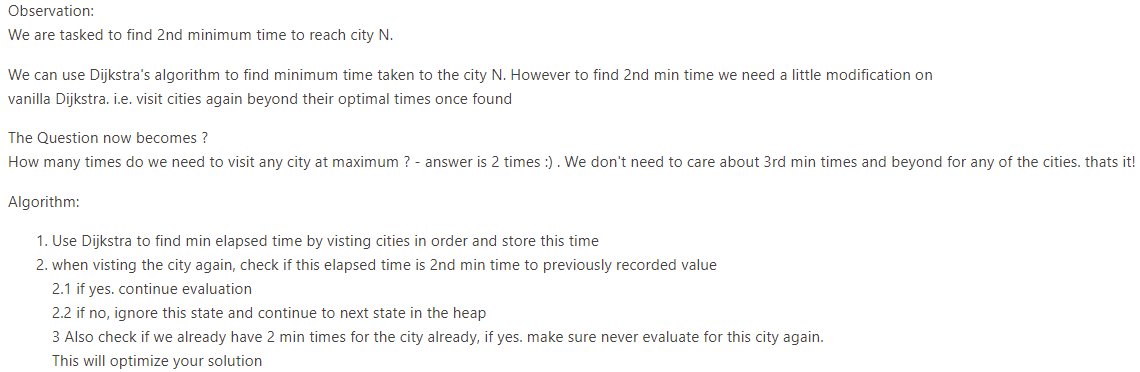
\includegraphics[width=.9\linewidth]{./pic/redGreen.png}

\begin{minted}[fontsize=\scriptsize,linenos=false]{csharp}
public int secondMinimum(int n, int[][] edges, int time, int change) {
    Map<Integer, List<Integer>> adj = new HashMap<>();
    for (int [] e : edges) {
        adj.computeIfAbsent(e[0], z -> new ArrayList<>()).add(e[1]);
        adj.computeIfAbsent(e[1], z -> new ArrayList<>()).add(e[0]);
    }
    Queue<int []> q = new PriorityQueue<>((a, b)->(a[1] -b[1]));
    q.offer(new int []{1, 0});
    Map<Integer, Integer> cache = new HashMap<>(); // use cache tmpo record min time per city
    // modification: we want to visit each city maximum two times with different times,
    // this will help in early termination when we visit the city again (3rd time or more)
    Set<Integer> exhausted = new HashSet<>();
    while (!q.isEmpty()) {
        int [] top = q.poll();
        int cur = top[0], t = top[1];
        // Base Termination : we have found our 2nd min time for city n
        if (cur == n && t > cache.getOrDefault(cur, Integer.MAX_VALUE))
            return t;
        if (!cache.containsKey(cur)) // we vistied this city for first time, so elapsed time is min for this city
            cache.put(cur, t);
        // early termination, if we are trying to visit the city 3rd time or more ,
        // or the elapsed time will not help in finding the solution
        else if (cache.get(cur) == t || exhausted.contains(cur)) continue;
        else // this means we are visiting the city with 2nd optimal time , we dont need to visit the city ever again
            exhausted.add(cur);
        // we visit the city on elapsedTime, we need to check if on basis of change time, whether this time falls in  cycle (green or red)
        // if odd cycle (red), we must wait for this cycle to end
        int factor = t / change;
        if (factor % 2 == 1)
            t = (factor + 1) * change;
        for (int nb : adj.getOrDefault(cur, new ArrayList<>())) { // visit the neighbours
            int visTime = t + time;
            if (!exhausted.contains(nb))
                q.offer(new int [] {nb, visTime});
        }
    }
    return -1;
}
\end{minted}
\begin{itemize}
\item 另一个也是写得直接了当的
\end{itemize}
\begin{minted}[fontsize=\scriptsize,linenos=false]{csharp}
public int secondMinimum(int n, int [][] edges, int time, int change) {
    Map<Integer, Set<Integer>> map = new HashMap<>();
    for (int [] e : edges) {
        map.computeIfAbsent(e[0], z -> new HashSet<>()).add(e[1]);
        map.computeIfAbsent(e[1], z -> new HashSet<>()).add(e[0]);
    }
    Queue<int []> q = new PriorityQueue<>((a, b)->(a[1]-b[1]));
    Map<Integer, Set<Integer>> vis = new HashMap<>();
    q.offer(new int [] {1, 0});
    int min = -1;
    while (!q.isEmpty()) {
        int [] top = q.poll();
        int cur = top[0], t = top[1];
        if (cur == n) {
            if (min == -1 || min == t) min = t;
            else return t;
        }
        if (t % (2 * change) >= change)
            t += 2 * change - t % (2 * change);
        // 源码中传入key和value,根据key获取看是否存在value,如果value==null,然后调用put方法把传入的key和value  put进map,返回根据key获取的老value
        // 如果传入key对应的value已经存在,就返回存在的value,不进行替换。如果不存在,就添加key和value,返回null
        vis.putIfAbsent(cur, new HashSet<>());
        if (!vis.get(cur).add(t) || vis.get(cur).size() >= 3) continue;
        if (map.containsKey(cur))
            for (int next : map.get(cur)) 
                q.offer(new int [] {next, t + time});
    }
    return -1;
}
\end{minted}

\subsection{1334. Floyd算法 - Find the City With the Smallest Number of Neighbors at a Threshold Distance - Medium}
\label{sec-1-1-4}
There are n cities numbered from 0 to n-1. Given the array edges where edges[i] = [fromi, toi, weighti] represents a bidirectional and weighted edge between cities fromi and toi, and given the integer distanceThreshold.

Return the city with the smallest number of cities that are reachable through some path and whose distance is at most distanceThreshold, If there are multiple such cities, return the city with the greatest number.

Notice that the distance of a path connecting cities i and j is equal to the sum of the edges' weights along that path.
\begin{minted}[fontsize=\scriptsize,linenos=false]{csharp}
public int findTheCity(int n, int[][] edges, int distanceThreshold) {
    // 1.创建邻接矩阵
    int [][] graph = new int [n][n]; // 相比于我只会用HashMap来建邻接关系,邻接链表与数组都可能,看哪个用起来方便
    for (int i = 0; i < n; i++)
        Arrays.fill(graph[i], Integer.MAX_VALUE); // pre filled n equaivlent to Integer.MAX_VALUE
    for (int [] eg : edges) {
        graph[eg[0]][eg[1]] = eg[2];
        graph[eg[1]][eg[0]] = eg[2];
    }
    // 2.floyd算法
    for (int k = 0; k < n; k++)          // 中间结点
        for (int i = 0; i < n; i++)      // 开始结点
            for (int j = 0; j < n; j++) {// 结尾结点
                if (i == j || graph[i][k] == Integer.MAX_VALUE || graph[k][j] == Integer.MAX_VALUE) continue;
                graph[i][j] = Math.min(graph[i][j], graph[i][k] + graph[k][j]);
            }                
    // 3.每个城市距离不大于distanceThreshold的邻居城市的数目
    int [] mark = new int [n]; //记录小于distanceThreshold的邻居城市个数
    for (int i = 0; i < n; i++) 
        for (int j = 0; j < n; j++) 
            if (graph[i][j] <= distanceThreshold)
                mark[i]++;
    // 4.找数目少,编号最大的
    int min = n;
    int ans = 0;
    for (int i = 0; i < n; i++) 
        if (min >= mark[i]) {
            min = mark[i];
            ans = i;
        }
    return ans;
}
\end{minted}
\begin{itemize}
\item 另一种解法
\end{itemize}
\begin{minted}[fontsize=\scriptsize,linenos=false]{csharp}
// 之前用原创想法也写了很多图的题,但缺乏归纳总结,原创想法更多的是解决了题目,但解法与效率、与优化算法间的距离还需要很多比较归纳与总结,才能把图这一块吃透
// https://leetcode.jp/leetcode-1334-find-the-city-with-the-smallest-number-of-neighbors-at-a-threshold-distance-%E8%A7%A3%E9%A2%98%E6%80%9D%E8%B7%AF%E5%88%86%E6%9E%90/  这个题需要重新写
// map:图结构
// city:当前城市
// dis:当前所剩距离
// v:已经被记录为邻居的节点
// maxDis:走到某个节点时,剩余距离的最大值
// 返回值为当前城市的邻居数。
private int dfs(int [][] arr, int city, int dis, boolean [] vis, int [] maxDis) {
    int res = 0;
    for (int i = 0; i < arr[0].length; i++) { // 循环当前城市的所有相邻城市
        int distance = arr[city][i]; // 与相邻城市的距离,如果为0,说明与该城市不相连
        int diffDis = dis - distance;// 到达相邻城市后,与阈值相比的剩余距离。
        if (distance > 0 && diffDis >= maxDis[i]) { // 与该城市相连并且剩余距离大于等于访问数组中的值
            maxDis[i] = diffDis;     // 更新访问数组中的剩余距离   
            if (!vis[i]) {
                vis[i] = true;
                res++;
            }
            res += dfs(arr, i, diffDis, vis, maxDis); // 递归dfs与该城市相连的其他城市:图中我似乎还很没有dfs以及递归的概念
        }
    }
    return res;
}
public int findTheCity(int n, int[][] edges, int distanceThreshold) {
    int [][] map = new int [n][n];
    for (int [] eg : edges) {
        map[eg[0]][eg[1]] = eg[2];
        map[eg[1]][eg[0]] = eg[2];
    }
    int min = n;
    int res = 0;
    for (int i = 0; i < n; i++) {
        boolean [] vis = new boolean [n];
        vis[i] = true;
        int cnt = dfs(map, i, distanceThreshold, vis, new int [n]);
        if (cnt <= min) {
            min = cnt;
            res = i;
        }
    }
    return res;
}
\end{minted}

\subsection{1129. Shortest Path with Alternating Colors - Medium}
\label{sec-1-1-5}
Consider a directed graph, with nodes labelled 0, 1, \ldots{}, n-1.  In this graph, each edge is either red or blue, and there could be self-edges or parallel edges.

Each [i, j] in red\_edges denotes a red directed edge from node i to node j.  Similarly, each [i, j] in blue\_edges denotes a blue directed edge from node i to node j.

Return an array answer of length n, where each answer[X] is the length of the shortest path from node 0 to node X such that the edge colors alternate along the path (or -1 if such a path doesn't exist).
\begin{minted}[fontsize=\scriptsize,linenos=false]{csharp}
// 找最短路径应该用queue来做,入队列的时候需要标记红边或是蓝边以便找交替路径
public int[] shortestAlternatingPaths(int n, int[][] red_edges, int[][] blue_edges) {
    HashMap<Integer, List<Integer>> [] maps = new HashMap [2]; // 0 : red; 1: blue
    for (int i = 0; i < 2; i++) 
        maps[i] = new HashMap<>();
    for (int i = 0; i < red_edges.length; i++) 
        maps[0].computeIfAbsent(red_edges[i][0], k->new ArrayList<>()).add(red_edges[i][1]);
    for (int i = 0; i < blue_edges.length; i++) 
        maps[1].computeIfAbsent(blue_edges[i][0], k->new ArrayList<>()).add(blue_edges[i][1]);
    int [] ans = new int[n];
    Arrays.fill(ans, -1);
    Queue<int []> q = new LinkedList<>();
    q.offer(new int [] {0, 0}); // red edge         
    q.offer(new int [] {0, 1}); // blue edge
    boolean [][] inQueue = new boolean [n][2]; // 0: red, 1: blue
    inQueue[0][0] = true;
    inQueue[0][1] = true;
    int cnt = 0, color = 0;
    while (!q.isEmpty()) {
        for (int size = q.size(); size > 0; size--) {
            int [] cur = q.poll();
            System.out.println(Arrays.toString(cur));
            color = cur[1];
            if (ans[cur[0]] == -1) ans[cur[0]] = cnt;
            List<Integer> nextNodes = maps[1-color].get(cur[0]);
            if (nextNodes == null) continue;
            for (Integer next : nextNodes) 
                if (!inQueue[next][1-color]) {
                    q.offer(new int [] {next, 1-color});
                    inQueue[next][1-color] = true;
                }
        }
        ++cnt;
    }
    return ans;
}
\end{minted}
\begin{itemize}
\item 不是总喜欢省掉大括号吗,试试省掉下面的。。。。。。
\end{itemize}
\begin{minted}[fontsize=\scriptsize,linenos=false]{csharp}
public int[] shortestAlternatingPaths(int n, int[][] red_edges, int[][] blue_edges) {
    int [][] red = new int[n][2]; // 红 0 蓝 1
    int [][] blue = new int[n][2];
    for (int i = 1; i < n; i++) {
        red[i][0] = i;
        red[i][1] = 0x0fffffff;   // 初始化红边权值
    }
    red [0][0] = 0;
    red [0][1] = 0;
    for (int i = 1; i < n; i++) {
        blue[i][0] = i;
        blue[i][1] = 0x0fffffff;
    }
    blue [0][0] = 0;
    blue [0][1] = 0;
    dfs(red, blue, 0, 0, red_edges, blue_edges);
    dfs(red, blue, 1, 0, red_edges, blue_edges);
    int [] ans = new int[n];
    for(int i = 0; i < n; i++){
        ans[i] = Math.min(red[i][1], blue[i][1]);
        if (ans[i] == 0x0fffffff) // 没有改变说明不存在
            ans[i] = -1;
    }
    return ans;
}
public void dfs(int [][] red, int [][] blue, int color, int node, int[][] red_edges, int[][] blue_edges){
    if (color == 0) { // 这个括号可以省吗???
        for (int [] blue_to : blue_edges) // 以node为from to 为终 的边
            if (node == blue_to[0] && red[node][1]+1 < blue[blue_to[1]][1]) {// 0到from点加1是否小于0到to的距离
                blue[blue_to[1]][1] = red[node][1]+1; // 作距离的更新
                dfs(red, blue, 1-color, blue_to[1], red_edges, blue_edges);
            }
    } else for (int [] red_to : red_edges) //以node为from to 为终 的边
               if (node == red_to[0] && blue[node][1]+1 < red[red_to[1]][1]) {//0到from点加1是否小于0到to的距离
                   red[red_to[1]][1] = blue[node][1]+1;
                   dfs(red, blue, 1-color, red_to[1], red_edges, blue_edges);
               }
}
\end{minted}

\subsection{882. Reachable Nodes In Subdivided Graph - Hard}
\label{sec-1-1-6}
You are given an undirected graph (the "original graph") with n nodes labeled from 0 to n - 1. You decide to subdivide each edge in the graph into a chain of nodes, with the number of new nodes varying between each edge.

The graph is given as a 2D array of edges where edges[i] = [ui, vi, cnti] indicates that there is an edge between nodes ui and vi in the original graph, and cnti is the total number of new nodes that you will subdivide the edge into. Note that cnti == 0 means you will not subdivide the edge.

To subdivide the edge [ui, vi], replace it with (cnti + 1) new edges and cnti new nodes. The new nodes are x1, x2, \ldots{}, xcnti, and the new edges are [ui, x1], [x1, x2], [x2, x3], \ldots{}, [xcnti-1, xcnti], [xcnti, vi].

In this new graph, you want to know how many nodes are reachable from the node 0, where a node is reachable if the distance is maxMoves or less.

Given the original graph and maxMoves, return the number of nodes that are reachable from node 0 in the new graph.

再进一步来分析,其实上对于每个结点来说(不论有没有编号),若我们能算出该结点离起始结点的最短距离,且该距离小于等于M的话,那这个结点就一定可以到达。这样来说,其实本质就是求单源点的最短距离,此时就要祭出神器迪杰斯特拉算法 Dijkstra Algorithm 了,LeetCode 中使用了该算法的题目还有 Network Delay Time 和 The Maze II。该算法的一般形式是用一个最小堆来保存到源点的最小距离,这里我们直接统计到源点的最小距离不是很方便,可以使用一个小 trick,即用一个最大堆来统计当前结点所剩的最大步数,因为剩的步数越多,说明距离源点距离越小。由于 Dijkstra 算法是以起点为中心,向外层层扩展,直到扩展到终点为止。根据这特性,用 BFS 来实现时再好不过了,首先来建立邻接链表,这里可以使用一个 NxN 的二维数组 graph,其中 graph[i][j] 表示从大结点i往大结点j方向会经过的小结点个数,建立邻接链表的时候对于每个 edge,要把两个方向都赋值,前面解释过了这里要当作有向图来做。然后使用一个最大堆,里面放剩余步数和结点编号组成的数对儿,把剩余步数放前面就可以默认按步数从大到小排序了,初始化时把 \{M,0\} 存入最大堆。还需要一个一维数组 visited 来记录某个结点是否访问过。

\begin{minted}[fontsize=\scriptsize,linenos=false]{csharp}
public int reachableNodes(int[][] edges, int maxMoves, int n) {
    int [][] graph = new int  [n][n];
    for (int i = 0; i < n; i++) 
        Arrays.fill(graph[i], -1);
    for (int [] v : edges) {
        graph[v[0]][v[1]] = v[2];
        graph[v[1]][v[0]] = v[2];
    }
    Queue<int []> q = new PriorityQueue<>((a, b) -> (b[0] - a[0]));
    boolean [] vis = new boolean [n];
    q.offer(new int [] {maxMoves, 0});
    int res = 0;
    while (!q.isEmpty()) {
        int [] cur = q.poll();
        int cnt = cur[0], u = cur[1];
        if (vis[u]) continue;
        vis[u] = true;
        ++res;
        for (int i = 0; i < n; i++) {
            if (graph[u][i] == -1) continue;
            if (cnt > graph[u][i] && !vis[i])
                q.offer(new int [] {cnt - graph[u][i]-1, i});
            graph[i][u] -= Math.min(cnt, graph[u][i]);
            res += Math.min(cnt, graph[u][i]);
        }
    }
    return res;
}
\end{minted}
\begin{itemize}
\item 我们也可以使用 HashMap 来建立邻接链表,最后的运行速度果然要比二维数组形式的邻接链表要快一些,其他的地方都不变,参见代码如下:
\end{itemize}
\begin{minted}[fontsize=\scriptsize,linenos=false]{csharp}
public int reachableNodes(int[][] edges, int maxMoves, int n) {
    int res = 0;
    Map<Integer, Map<Integer, Integer>> graph = new HashMap<>();
    for (int [] v : edges) {
        graph.computeIfAbsent(v[0], k->new HashMap<>()).put(v[1], v[2]);
        graph.computeIfAbsent(v[1], k->new HashMap<>()).put(v[0], v[2]);
    }
    Queue<int []> q = new PriorityQueue<>((a, b) -> (b[0] - a[0]));
    boolean [] vis = new boolean [n];
    q.offer(new int [] {maxMoves, 0});
    while (!q.isEmpty()) {
        int [] cur = q.poll();
        int cnt = cur[0], u = cur[1];
        if (vis[u]) continue;
        vis[u] = true;
        ++res;
        for (int i = 0; i < n; i++) {
            if (!graph.containsKey(u) || !graph.get(u).containsKey(i) || graph.get(u).get(i) == -1) continue;
            if (cnt > graph.get(u).get(i) && !vis[i])
                q.offer(new int [] {cnt - graph.get(u).get(i)-1, i});
            graph.get(i).put(u, graph.get(u).get(i) - Math.min(cnt, graph.get(u).get(i)));
            res += Math.min(cnt, graph.get(u).get(i));
        }
    }
    return res;
}
\end{minted}

\subsection{1782. Count Pairs Of Nodes - Hard}
\label{sec-1-1-7}
You are given an undirected graph defined by an integer n, the number of nodes, and a 2D integer array edges, the edges in the graph, where edges[i] = [ui, vi] indicates that there is an undirected edge between ui and vi. You are also given an integer array queries.

Let incident(a, b) be defined as the number of edges that are connected to either node a or b.

The answer to the jth query is the number of pairs of nodes (a, b) that satisfy both of the following conditions:

a < b
incident(a, b) > queries[j]
Return an array answers such that answers.length == queries.length and answers[j] is the answer of the jth query.

Note that there can be multiple edges between the same two nodes.
\begin{minted}[fontsize=\scriptsize,linenos=false]{csharp}
// https://leetcode.com/problems/count-pairs-of-nodes/discuss/1096740/C%2B%2BJavaPython3-Two-Problems-O(q-*-(n-%2B-e))
public int[] countPairs(int n, int[][] edges, int[] queries) { // 别人家的思路好清晰
    int [] cnt = new int [n+1], sortedCnt = new int [n+1], ans = new int [queries.length];
    Map<Integer, Integer> [] m = new HashMap[n+1];
    for (var e : edges) {
        sortedCnt[e[0]] = cnt[e[0]] = cnt[e[0]] + 1;
        sortedCnt[e[1]] = cnt[e[1]] = cnt[e[1]] + 1;
        int min = Math.min(e[0], e[1]), max = Math.max(e[0], e[1]);
        m[min] = m[min] == null ? new HashMap<>() : m[min];
        m[min].put(max, m[min].getOrDefault(max, 0) + 1); // 仍然是当作有向图、单向图来做
    }
    Arrays.sort(sortedCnt);
    int res = 0, cur = 0;
    for (int k = 0; k < queries.length; k++) {
        for (int i = 1, j = n; i < j;) 
            if (queries[k] < sortedCnt[i] + sortedCnt[j])
                ans[k] += (j--) - i;
            else ++i;
        for (int i = 1; i <= n; i++) 
            if (m[i] != null) 
                for (var en : m[i].entrySet()) {
                    int j = en.getKey(), sharedCnt = en.getValue();
                    if (queries[k] < cnt[i] + cnt[j] && cnt[i] + cnt[j] - sharedCnt <= queries[k])
                        ans[k]--;
                }
    } 
    return ans;
}
\end{minted}

\subsection{2115. Find All Possible Recipes from Given Supplies}
\label{sec-1-1-8}
You have information about n different recipes. You are given a string array recipes and a 2D string array ingredients. The ith recipe has the name recipes[i], and you can create it if you have all the needed ingredients from ingredients[i]. Ingredients to a recipe may need to be created from other recipes, i.e., ingredients[i] may contain a string that is in recipes.

You are also given a string array supplies containing all the ingredients that you initially have, and you have an infinite supply of all of them.

Return a list of all the recipes that you can create. You may return the answer in any order.

Note that two recipes may contain each other in their ingredients.
\begin{enumerate}
\item 解题思路与分析
\label{sec-1-1-8-1}
\begin{minted}[fontsize=\scriptsize,linenos=false]{csharp}
public List<String> findAllRecipes(String[] re, List<List<String>> ing, String[] sup) { // 菜谱 菜谱原材料 食材 BUG BUG BUG
    Map<String, Set<String>> adj = new HashMap<>();    // 每种材料可以做成的菜的 清单
    Map<String, Integer> ins = new HashMap<>();        // 每种材料或是菜谱的 入度
    for (int i = 0; i < re.length; i++) 
        for (String it : ing.get(i)) {
            adj.computeIfAbsent(it, z -> new HashSet<>()).add(re[i]);
            ins.put(re[i], ins.getOrDefault(re[i], 0) + 1);
        }
    List<String> ans = new ArrayList<>();
    Deque<String> q = new ArrayDeque<>();
    for (String s : sup) q.offerLast(s); // 把初始的原材料放入队列
    while (!q.isEmpty()) { // 拓扑排序
        String cur = q.pollFirst();
        if (adj.containsKey(cur)) 
            for (String one : adj.get(cur)) { // 遍历某种原材料可以做成的所有的菜,其入度是否为0
                ins.put(one, ins.get(one)-1); // 入度 ins--
                if (ins.get(one) == 0) {
                    ans.add(one);
                    q.offerLast(one);
                }
            }
    }
    return ans;
}
\end{minted}
\end{enumerate}

\section{基环内向树}
\label{sec-1-2}
\subsection{2127. Maximum Employees to Be Invited to a Meeting - Hard 基环内向树}
\label{sec-1-2-1}
A company is organizing a meeting and has a list of n employees, waiting to be invited. They have arranged for a large circular table, capable of seating any number of employees.

The employees are numbered from 0 to n - 1. Each employee has a favorite person and they will attend the meeting only if they can sit next to their favorite person at the table. The favorite person of an employee is not themself.

Given a 0-indexed integer array favorite, where favorite[i] denotes the favorite person of the ith employee, return the maximum number of employees that can be invited to the meeting.
\begin{enumerate}
\item 解题思路与分析
\label{sec-1-2-1-1}
如果我们把每个员工看成图上的一个节点,如果员工 xx 喜欢员工 yy,就在从 xx 对应的节点到 yy 对应的节点连一条边,那么形成的图是什么结构的?形成的图会由若干颗「基环内向树」组成。所谓「基环内向树」,就是形如下图所示的结构:

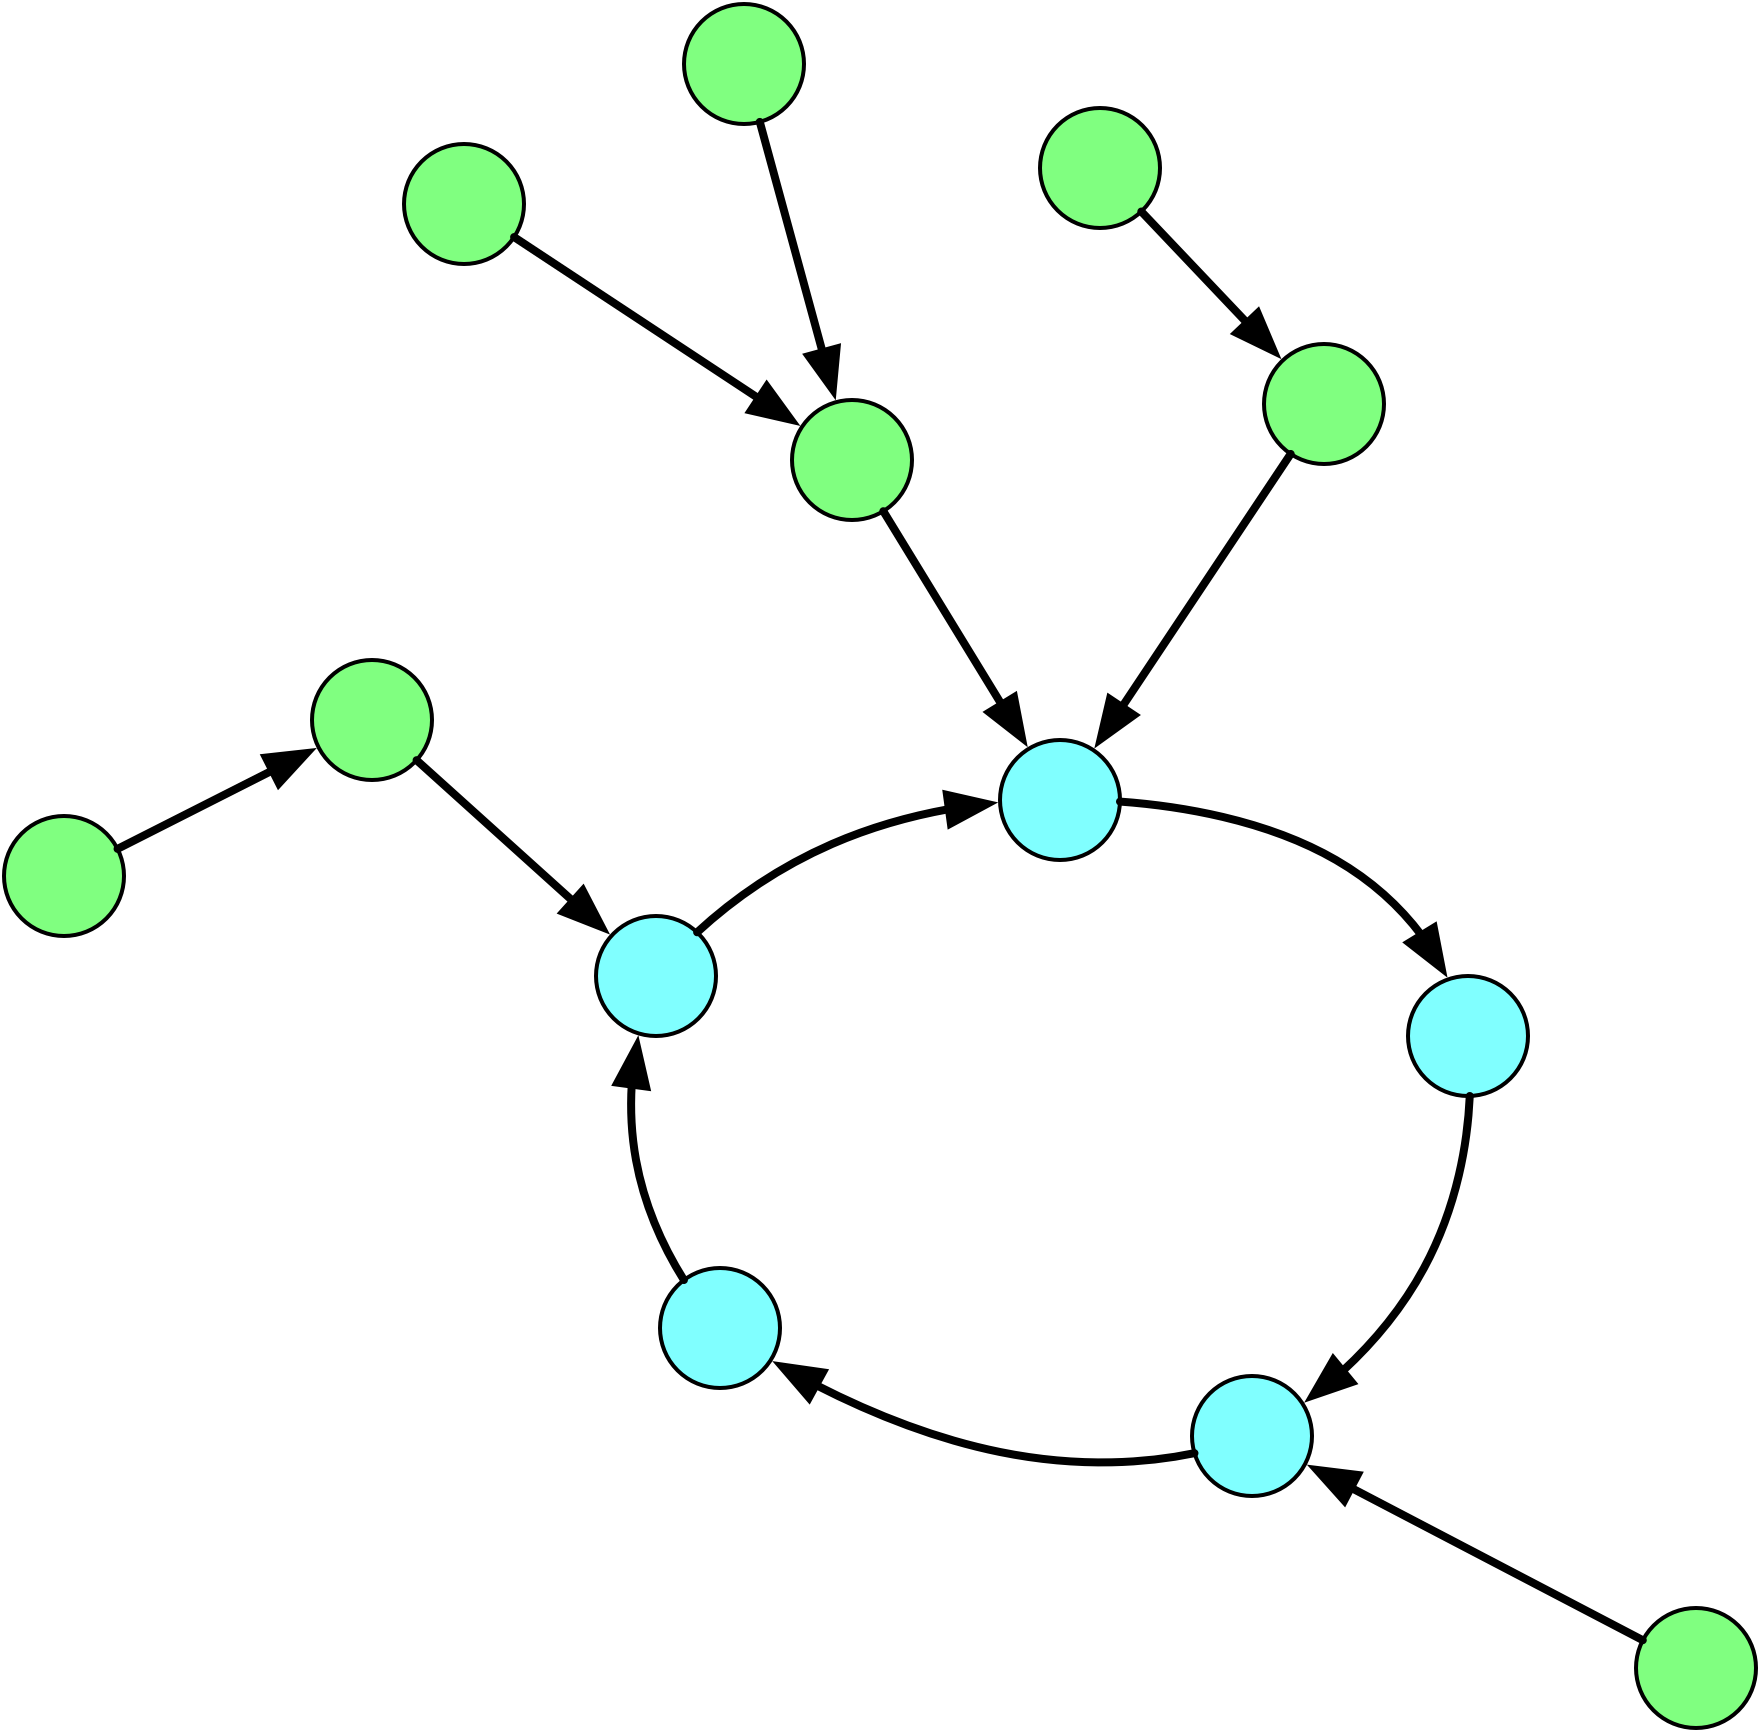
\includegraphics[width=.9\linewidth]{./pic/2277tree-1.png}


我们从任意一个节点 xx 开始在图上进行「游走」,由于每个员工只有一位喜欢的员工,因此每个节点在图上只会有一条出边,即「游走」的过程是唯一的。由于图上有 nn 个节点,因此在 n+1n+1 步以内,一定会走到一个重复的节点,那么在第一次经过该节点之后,到第二次经过该节点之前的所有节点,以及该节点本身,就组成了一个环,如上图的蓝色节点所示。

对于不在环上的节点,我们已经说明了从它们开始「游走」也一定会进入到环中。在到达环上的节点之前,它们不会重复经过节点(否则就有两个环了,我们可以证明一个连通分量中是不可能有两个环的:因为每个节点只有一条出边,因此如果有两个环并且它们连通,那么必然某个环上有一个点有两条出边,一条出边指向同一个环上的节点,另一条出边可以使得它到达另一个环,这就产生了矛盾),那么它们就形成了类似树的结构,如上图的绿色节点所示。

需要注意的是,一个单独的环也是「基环内向树」,它是一种特殊情况,即没有绿色的节点。

思路与算法

既然我们知道了图由若干颗「基环内向树」组成,那么我们就可以想一想,每一颗「基环内向树」的哪一部分可以被安排参加会议。

我们首先讨论特殊的情况,即一个单独的环(或若干个环),并且所有环的大小都 $\ge$ 3≥3。可以发现,我们按照环上的顺序给对应的员工安排座位是满足要求的,因为对于每一个环上的员工,它喜欢的员工就在它的旁边。并且,我们必须安排环上的所有员工,因为如果有缺失,那么喜欢那位缺失了的员工的员工就无法满足要求了。

但如果我们已经安排了某一个环上的所有员工,剩余的环就没有办法安排了。这是因为已经安排的那个环是没有办法被「断开」的:断开的本质就是相邻位置员工的缺失。因此,我们可以得出一个重要的结论:

如果我们想安排大小 $\ge$ 3≥3 的环,我们最多只能安排一个,并且环需要是完整的。

那么如果是环大小 $\ge$ 3≥3 的「基环内向树」呢?如果我们安排了不在环上的节点,那么从该节点开始,我们需要不断安排当前节点喜欢的员工,这实际上就是「游走」的过程。而当我们游走到环上并到达环上最后一个未经过的节点时,该节点的下一个节点(即喜欢的员工)已经被安排过,所以最后一个未经过的节点就无法被安排,不满足要求。因此,我们不能安排任何不在环上的节点,只能安排在环上的节点,就得出了另一个的结论:

所有环大小 $\ge$ 3≥3 的「基环内向树」与一个大小相同(指环的部分)的环是等价的。

那么最后我们只需要考虑大小 =2=2 的环或者「基环内向树」了。这里的特殊之处在于,大小 =2=2 的环可以安排多个:因为环上的两个点是互相喜欢的,因此只需要它们相邻即可,而没有其它的要求。而对于环大小 =2=2 的「基环内向树」,如果我们安排了不在环上的节点,那么游走完环上两个节点之后,同样是满足要求的,并且我们甚至可以继续延伸(反向「游走」),到另一个不在环上的节点为止。如下图所示,包含 \texttt{X}X 的节点就是可以安排参加会议的节点。

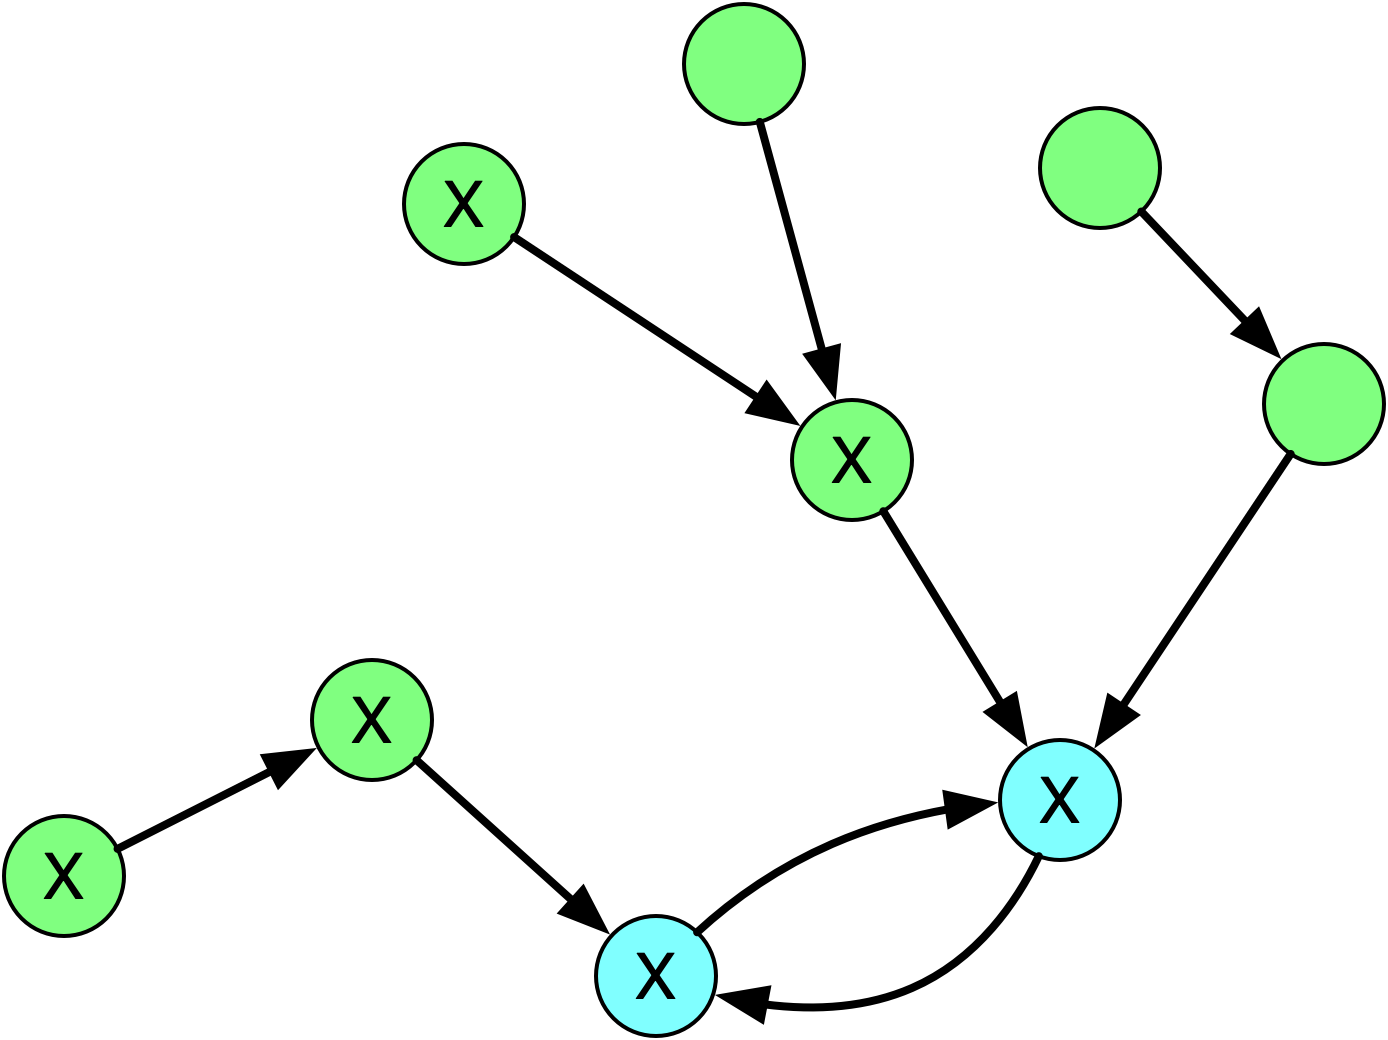
\includegraphics[width=.9\linewidth]{./pic/2277tree-2.png}

并且同样地,对于每一棵环大小 =2=2 的「基环内向树」,我们都可以取出这样一条「双向游走」路径进行安排,它们之间不会影响。综上所述,原问题的答案即为下面二者中的最大值:

最大的环的大小;

所有环大小 =2=2 的「基环内向树」上的最长的「双向游走」路径之和。

为了求解「基环内向树」上的最长的「双向游走」路径,我们可以使用拓扑排序 + 动态规划的方法。记 f[i]f[i] 表示到节点 ii 为止的最长「游走」路径经过的节点个数,那么状态方程即为:

即我们考虑节点 ii 的上一个节点 jj,在图中必须有从 jj 到 ii 的一条有向边,这样我们就可以从 jj 转移到 ii。如果不存在满足要求的 jj(例如「基环内向树」退化成一个大小 =2=2 的环),那么 f[i] = 1f[i]=1。状态转移可以和拓扑排序同时进行。

在拓扑排序完成后,剩余没有被弹出过队列的节点就是环上的节点。我们可以找出每一个环。如果环的大小 $\ge$ 3≥3,我们就用其来更新最大的环的大小;如果环的大小 =2=2,设环上的两个节点为 xx 和 yy,那么该「基环内向树」上最长的「双向游走」的路径长度就是 f[x] + f[y]f[x]+f[y]。

\begin{minted}[fontsize=\scriptsize,linenos=false]{csharp}
public int maximumInvitations(int[] a) { // a: favorite
    // 统计入度,便于进行拓扑排序
    int n = a.length, ins [] = new int [n];
    for (int v : a) ins[v]++;
    boolean vis [] = new boolean [n];
    int f [] = new int [n];
    Arrays.fill(f, 1);
    Deque<Integer> q = new ArrayDeque<>();
    for (int i = 0; i < n; i++) 
        if (ins[i] == 0) q.offerLast(i); 
    while (!q.isEmpty()) {
        int u = q.pollFirst();
        vis[u] = true;
        int v = a[u];
        f[v] = Math.max(f[v], f[u] + 1); // 动态规划: 能够到达 v 的最长链的长度
        --ins[v];
        if (ins[v] == 0) q.offerLast(v);
    }
    // ring 表示最大的环的大小
    // total 表示所有环大小为 2 的「基环内向树」上的最长的「双向游走」路径之和
    int ring = 0, total = 0;
    for (int i = 0; i < n; i++) {
        if (!vis[i]) {
            int j = a[i];
            if (a[j] == i) { // 说明环的大小为 2
                total += f[i] + f[j]; // 局部二元环可以叠加
                vis[i] = vis[j] = true;
            } else { // 否则环的大小至少为 3,我们需要找出环
                int u = i, cnt = 0;
                do { // 至少执行一次,evaluate after execute
                    ++cnt;
                    u = a[u];
                    vis[u] = true;
                } while (u != i); // 再达到达这一点,说明转了一圈,又回到了起点
                ring = Math.max(ring, cnt); // 找出一个节点数目最多的环
            }
        }
    }
    return Math.max(ring, total);
}
\end{minted}
\end{enumerate}
\section{Tarjan 算法}
\label{sec-1-3}
\begin{itemize}
\item 图的一些基本概念:
\item \textbf{关联(incident)} : 点为边的端点;
\item \textbf{邻接(adjacent)} : 点与点关联同一条边,或边与边关联同一顶点;
\item \textbf{子图} : 图G'的点和边都是图G的子集,则G'为G的子图;
\item \textbf{道路} : 从点v到点u的路径;
\begin{itemize}
\item \textbf{简单道路} : 没有重复边的道路;
\item \textbf{回路} : 起点与终点相同的道路;
\item \textbf{简单回路} : 没有重复边的回路;
\item \textbf{连通} : 两顶点间有道路;
\item \textbf{强连通} : 有向图u→v与v→u都有道路;
\item \textbf{连通图} : 任意两顶点间都有道路(若有向图除去方向后连通,则称有向图连通);
\item \textbf{简单图} : 没有重复边和自环的图;
\item \textbf{完全图} : 任意两顶点间有一条边到达的简单图(有向完全图与无向完全图);
\item \textbf{强连通(strongly connected)} : 在有向图G 中,如果两个顶点间至少存在一条路径,称两个顶点强连通(strongly connected);
\item \textbf{强连通图} : 如果有向图G 的每两个顶点都强连通,称G 是一个强连通图;
\item \textbf{强连通分量(strongly connected components)} : 非强连通图有向图的极大强连通子图,称为强连通分量(strongly connected components)。
\end{itemize}
\item 无向图的割点与桥
\begin{itemize}
\item 什么是无向图?简单来说,若一个图中每条边都是无方向的,则称为无向图。
\item 割点: 若从图中删除节点 x 以及所有与 x 关联的边之后,图将被分成两个或两个以上的不相连的子图,那么称 x 为图的割点。
\item 桥: 若从图中删除边 e 之后,图将分裂成两个不相连的子图,那么称 e 为图的桥或割边。
\end{itemize}
\item 求强连通分量就是我们今天要解决的问题,根据强连通分量定义,用双向遍历取交集的方法求强连通分量,时间复杂度为O(\$N\^{}2\$+M). 而Tarjan或Kosaraju算法, 两者的时间复杂度都是O(N+M)。
\end{itemize}
\subsection{算法简介}
\label{sec-1-3-1}

在了解了 Tarjan 算法的背景以及图的割点与桥的基本概念之后,我们下面所面临的问题就是 —— 如何求解图的割点与桥?

开门见山,我们直接引出 Tarjan 算法在求解无向图的割点与桥的工作原理。

\begin{itemize}
\item 时间戳: ​时间戳是用来标记图中每个节点在进行深度优先搜索时被访问的时间顺序,当然,你可以理解成一个序号(这个序号由小到大),用 dfn[x] 来表示。
\item 搜索树: 在无向图中,我们以某一个节点 x 出发进行深度优先搜索,每一个节点只访问一次,所有被访问过的节点与边构成一棵树,我们可以称之为“无向连通图的搜索树”。
\item 追溯值: 追溯值用来表示从当前节点 x 作为搜索树的根节点出发,能够访问到的所有节点中,时间戳最小的值 —— low[x]。那么,我们要限定下什么是“能够访问到的所有节点”?,其需要满足下面的条件之一即可:
\begin{itemize}
\item 以 x 为根的搜索树的所有节点
\item 通过一条非搜索树上的边,能够到达搜索树的所有节点
\end{itemize}
\end{itemize}

Tarjan 算法是基于对图深度优先搜索的算法,每个强连通分量为搜索树中的一棵子树。搜索时,把当前搜索树中未处理的节点加入一个堆栈,回溯时可以判断栈顶到栈中的节点是否为一个强连通分量。

\begin{itemize}
\item 定义:
\begin{itemize}
\item o DFN(u)为节点u 搜索的次序编号(时间戳);
\item o LOW(u)为u 或 u的子树能够追溯到的最早的栈中节点的次序号;
\end{itemize}
\end{itemize}

由定义可以得出,当 DFN(u)=LOW(u)时,以u为根的搜索子树上所有节点是一个强连通分量。

\begin{itemize}
\item 算法:
\begin{itemize}
\item 当首次搜索到点u时DFN[u]=LOW[u]=time;
\item 每当搜索到一个点,把该点压入栈顶;
\item 当u和v有边相连时:
\end{itemize}
\end{itemize}

1)如果v不在栈中(树枝边),DFS(v),并且LOW[u] = min\{LOW(u),LOW(v)\};

2)如果v在栈中(前向边/后向边),此时LOW[u] = min\{LOW[u],DFN[v]\}
\begin{itemize}
\item 当DFN[u]=LOW[u]时,将它以及在它之上的元素弹出栈,此时,弹出栈的结点构成一个强连通分量;
\item 继续搜索,知道图被遍历完毕。
\end{itemize}

由于在这个过程中每个点只被访问一次,每条边也只被访问一次,所以Tarjan算法的时间复杂度是O(n+m).

\begin{itemize}
\item 这个算法需要用到好几个辅助数组, 下面我来详细介绍它们的作用
\begin{itemize}
\item int dfn[MAXN];// 用来记录一个顶点第一次被访问时的时间戳
\item int low[MAXN];// 用来记录一个顶点不经过它的父亲顶点最高能访问到它的祖先节点中的最小时间戳, 通俗易懂的来说, 就是与结点i连接的所有点中dfn[]值最小的一个。
\item int cut[MAXN];// 用来记录该点是否是割点, 因为一个割点可能多次被记录
\end{itemize}
\end{itemize}

\subsection{1192. Critical Connections in a Network- Hard Tarjan 算法 Tarjan's algorithm Kosaraju算法 -- todo: 这个题不太懂}
\label{sec-1-3-2}
There are n servers numbered from 0 to n - 1 connected by undirected server-to-server connections forming a network where connections[i] = [ai, bi] represents a connection between servers ai and bi. Any server can reach other servers directly or indirectly through the network.

A critical connection is a connection that, if removed, will make some servers unable to reach some other server.

Return all critical connections in the network in any order.
\begin{enumerate}
\item 解题思路与分析
\label{sec-1-3-2-1}
\begin{itemize}
\item \url{https://www.cnblogs.com/nullzx/p/7968110.html}

\begin{minted}[fontsize=\scriptsize,linenos=false]{csharp}
public List<List<Integer>> criticalConnections(int n, List<List<Integer>> connections) {
    depth = new int [n];
    Arrays.fill(depth, -1);
    adj = new ArrayList[n]; // 初始化结构图map[i]代表节点i可以连通哪些节点
    for (int i = 0; i < n; i++) adj[i] = new ArrayList<>();
    for (List<Integer> c : connections) {
        adj[c.get(0)].add(c.get(1));
        adj[c.get(1)].add(c.get(0));
    }
    dfs(0, 0, 0);
    return ans;
}
List<List<Integer>> ans = new ArrayList<>();
List<Integer> [] adj;
int [] depth;
int dfs(int cur, int pre, int dep) { // 返回值为当前节点所有dfs路径终点的最小深度
    depth[cur] = dep; // 将当前深度存入深度数组
    int res = Integer.MAX_VALUE;
    for (int v : adj[cur]) {
        if (v == pre) continue;
        int endDepth; // dfs终点深度
        if (depth[v] == -1) {
            endDepth = dfs(v, cur, dep + 1);
            // 如果深度大于当前深度,说明当前点不在闭环上, 当前点与下一节点i之间的连线为答案之一
            if (endDepth > dep)
                ans.add(List.of(cur, v));
        } else endDepth = depth[v];
        res = Math.min(res, endDepth);
    }
    return res;
}
\end{minted}
\end{itemize}
\end{enumerate}

\section{无向图}
\label{sec-1-4}
\subsection{2508. Add Edges to Make Degrees of All Nodes Even}
\label{sec-1-4-1}
There is an undirected graph consisting of n nodes numbered from 1 to n. You are given the integer n and a 2D array edges where edges[i] = [ai, bi] indicates that there is an edge between nodes ai and bi. The graph can be disconnected.

You can add at most two additional edges (possibly none) to this graph so that there are no repeated edges and no self-loops.

Return true if it is possible to make the degree of each node in the graph even, otherwise return false.

The degree of a node is the number of edges connected to it.
\begin{enumerate}
\item 怎么才能把问题分析透彻,看清问题考查的本质
\label{sec-1-4-1-1}

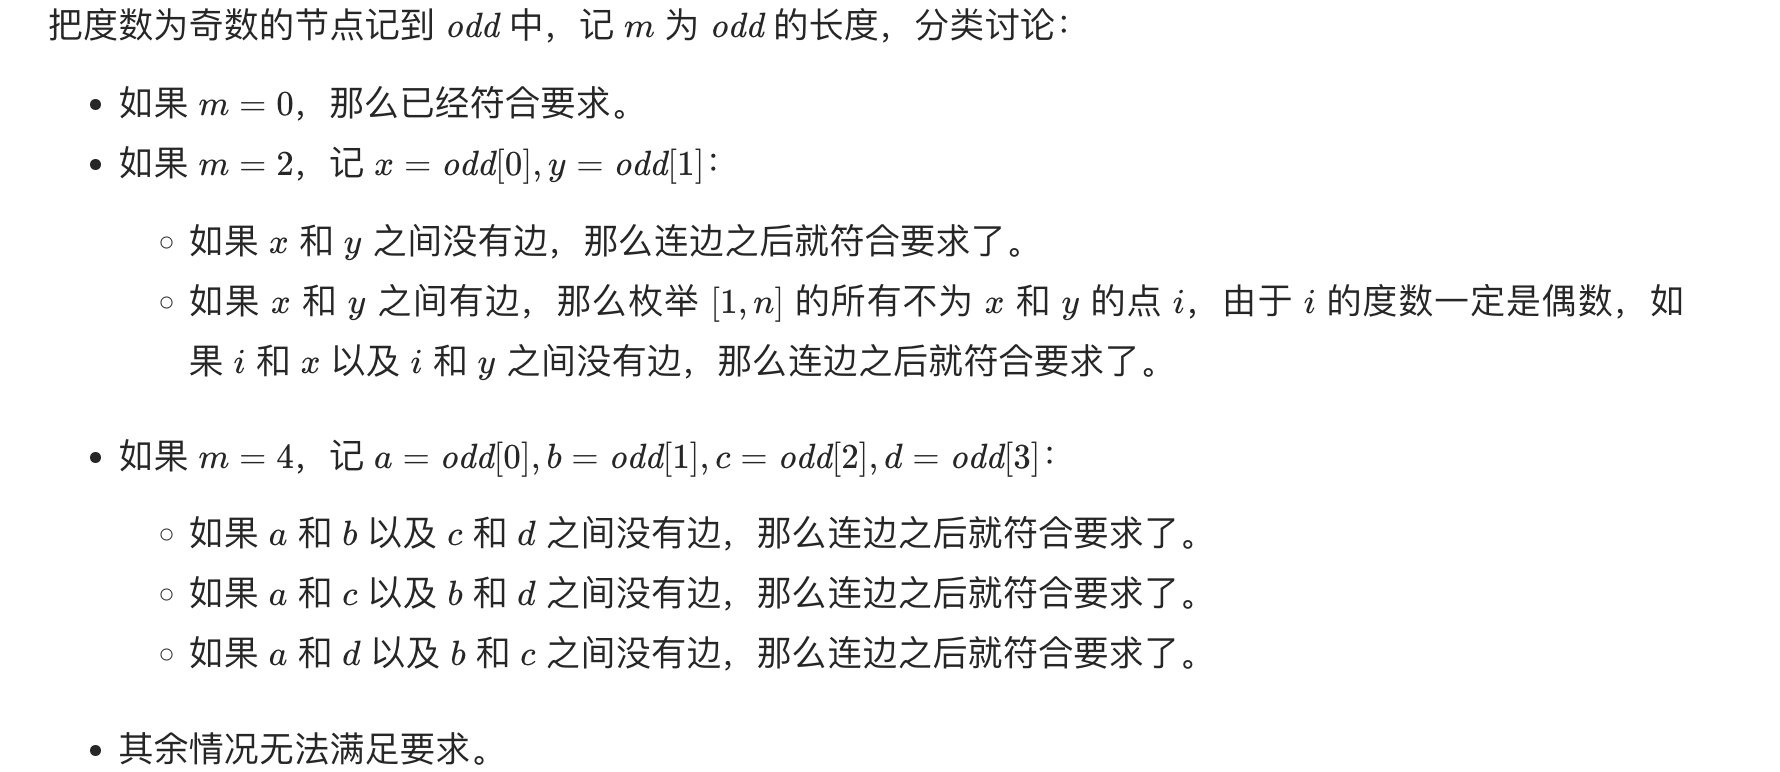
\includegraphics[width=.9\linewidth]{./pic/graph_20230412_083249.png}
\begin{minted}[fontsize=\scriptsize,linenos=false]{java}
public boolean isPossible(int n, List<List<Integer>> edges) {
    // 【建图】
    var g = new Set [n+1];
    Arrays.setAll(g, e -> new HashSet<Integer>()); // 初始化
    for (var e : edges) {
        int u = e.get(0), v = e.get(1);
        g[u].add(v);
        g[v].add(u);
    }
    // 【数与列举:度数为奇数的节点】
    var odd = new ArrayList<Integer>();
    for (int i = 1; i <= n; i++) 
        if (g[i].size() % 2 > 0) odd.add(i);
    var m = odd.size();
    // 【对度数为奇数的节点,结果,进行分析】
    if (m == 0) return true;
    if (m == 2) {
        int x = odd.get(0), y = odd.get(1);
        if (!g[x].contains(y)) return true;
        for (int i = 1; i <= n; i++) 
            if (i != x && i != y && !g[x].contains(i) && !g[y].contains(i)) return true;
        return false;
    }
    if (m == 4) {
        int x = odd.get(0), y = odd.get(1), i = odd.get(2), j = odd.get(3);
        return !g[x].contains(y) && !g[i].contains(j) // [a, b], [c, d]
            || !g[x].contains(i) && !g[y].contains(j) // [a, c], [b, d]
            || !g[x].contains(j) && !g[y].contains(i);// [a, d], [b, c]
    }
    return false;
}
\end{minted}
\end{enumerate}
\subsection{2538. Difference Between Maximum and Minimum Price Sum}
\label{sec-1-4-2}
There exists an undirected and initially unrooted tree with n nodes indexed from 0 to n - 1. You are given the integer n and a 2D integer array edges of length n - 1, where edges[i] = [ai, bi] indicates that there is an edge between nodes ai and bi in the tree.

Each node has an associated price. You are given an integer array price, where price[i] is the price of the ith node.

The price sum of a given path is the sum of the prices of all nodes lying on that path.

The tree can be rooted at any node root of your choice. The incurred cost after choosing root is the difference between the maximum and minimum price sum amongst all paths starting at root.

Return the maximum possible cost amongst all possible root choices.
\begin{enumerate}
\item 基本分析
\label{sec-1-4-2-1}

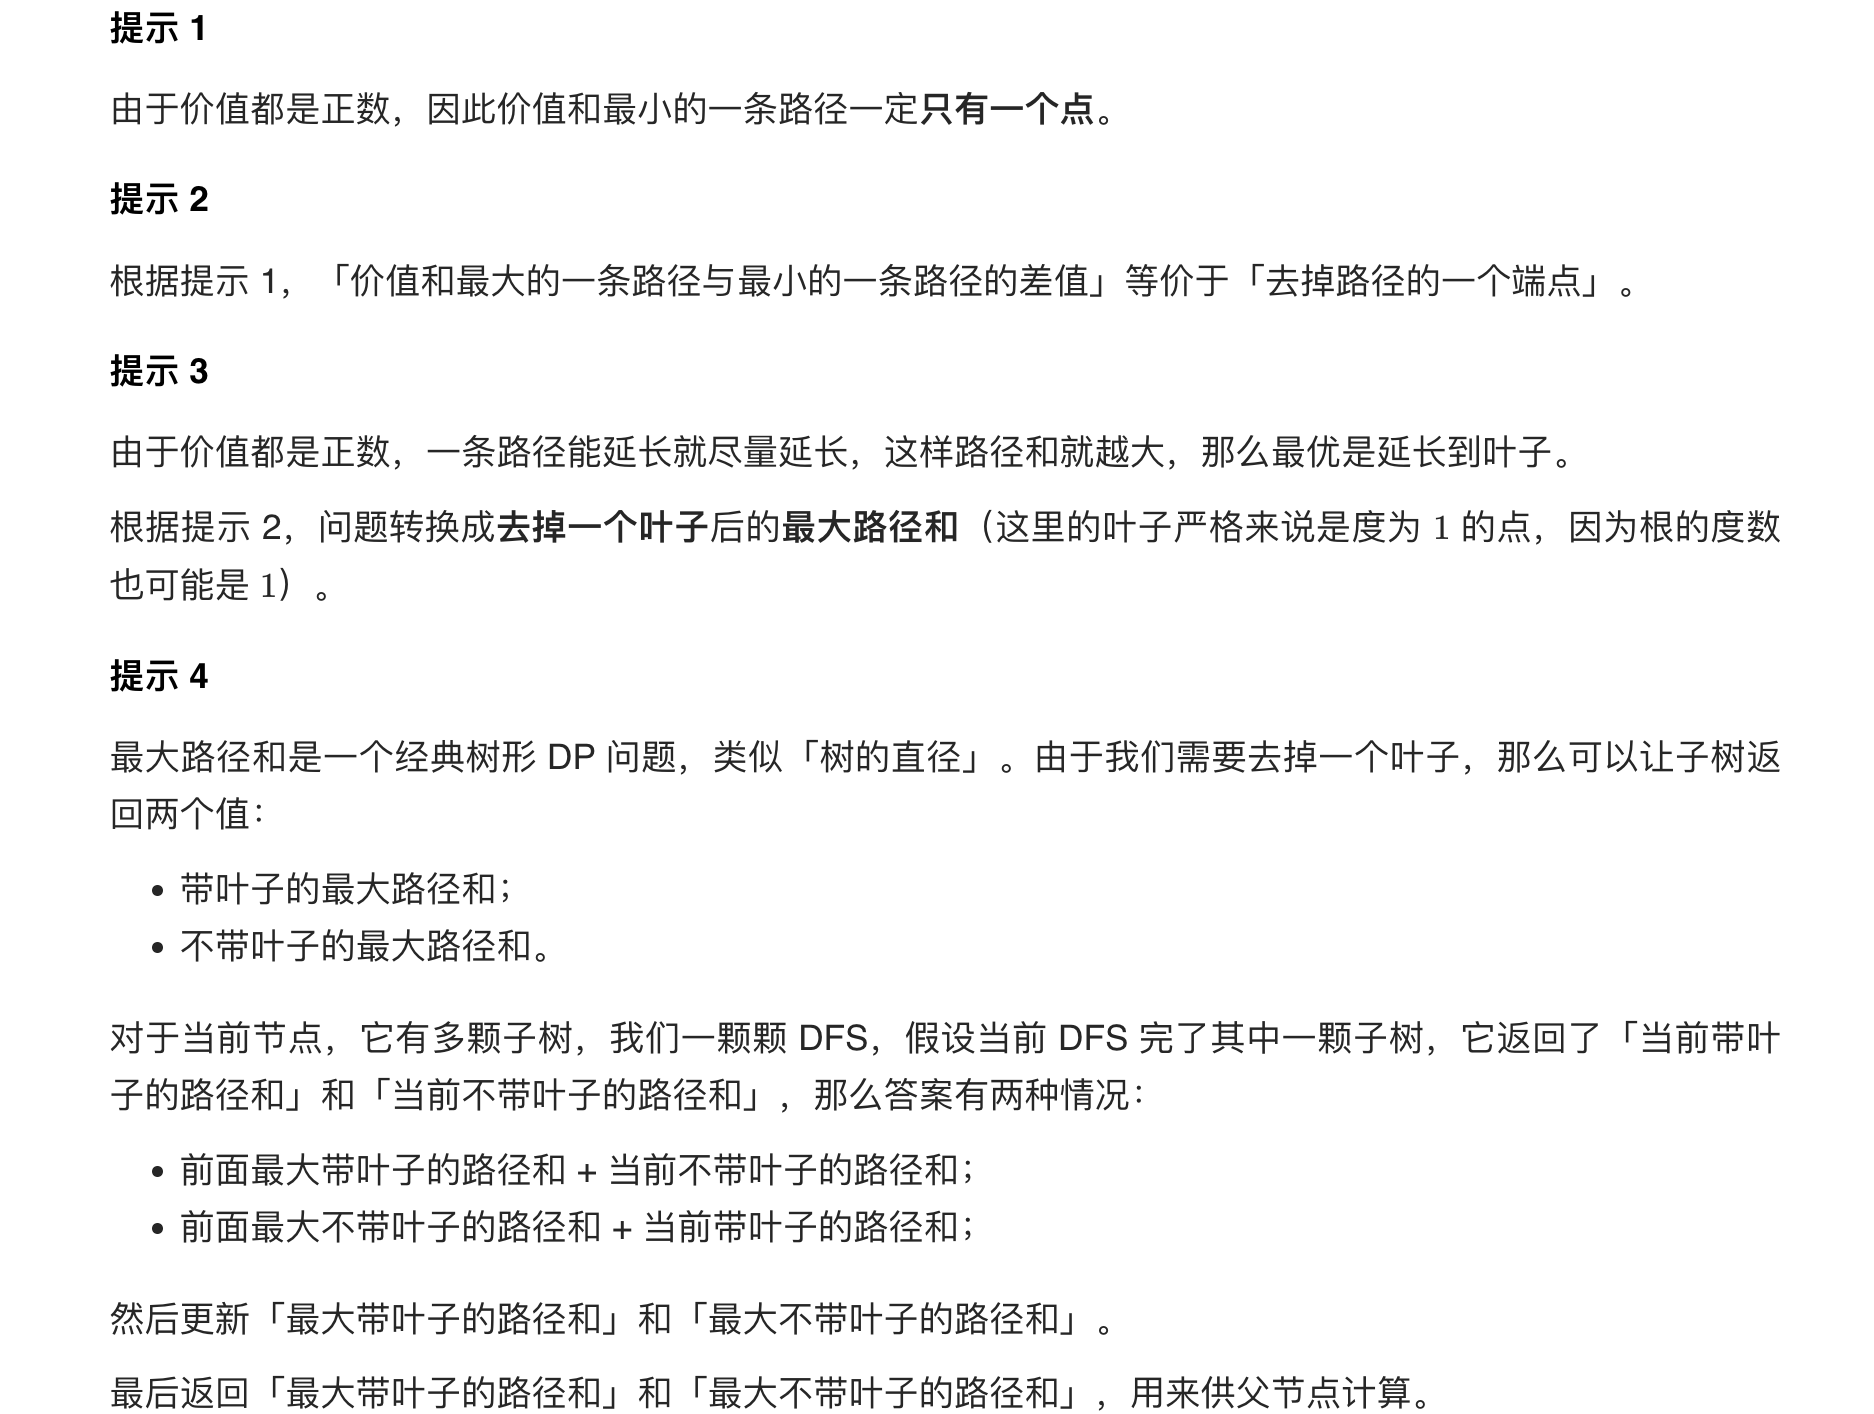
\includegraphics[width=.9\linewidth]{./pic/graph_20230412_132942.png}
\begin{minted}[fontsize=\scriptsize,linenos=false]{java}
public long maxOutput(int n, int[][] edges, int[] price) {
    g = new ArrayList [n];
    Arrays.setAll(g, x -> new ArrayList<>());
    for (int [] e : edges) {
        int x = e[0], y = e[1];
        g[x].add(y);
        g[y].add(x);
    }
    dfs(0, -1, price);
    return ans;
}
List<Integer> [] g;
long ans;
// 返回【带叶子的最大路径和,不带叶子的最大路径和】
long [] dfs(int x, int fa, int [] price) {
    long p = price[x], maxSone = p, maxStwo = 0;
    for (int v : g[x]) 
        if (v != fa) {
            var res = dfs(v, x, price);
            long s = res[0], ss = res[1];
            // 前面最大  带叶子的路径和 + 当前不带叶子的路径和【  带 + 不带】
            // 前面最大不带叶子的路径和 + 当前  带叶子的路径和【不带 +   带】
            ans = Math.max(ans, Math.max(maxSone + ss, maxStwo + s));
            maxSone = Math.max(maxSone, s + p);
            maxStwo = Math.max(maxStwo, ss + p); // 这里加上 p 是因为 x 必然不是叶子【什么情况下是叶了的情况,我没想清楚】
        }
    return new long [] {maxSone, maxStwo};
}
\end{minted}
\end{enumerate}
\section{欧拉回路: Hierholzer 算法, Fleury算法}
\label{sec-1-5}
\begin{itemize}
\item AOV\&AOE
\item AOVAOV网,顶点表示活动,弧表示活动间的优先关系的有向图。 即如果a->b,那么a是b的先决条件。
\item AOEAOE网,边表示活动,是一个带权的有向无环图, 其中顶点表示事件,弧表示活动,权表示活动持续时间。
\end{itemize}

求拓扑序列就是AOVAOV,求关键路径就是AOEAOE

入度: 入度(indegree)就是有向图中指向这个点的边的数量,即有向图的某个顶点作为终点的次数和

出度: 出度(outdegree)就是从这个点出去的边的数量,即有向图的某个顶点作为起点的次数和

\begin{itemize}
\item 定义
\begin{itemize}
\item 欧拉回路(Eulerian Circuit):从图上一个点u出发不重复地经过每一条边后,再次回到点u的一条路径。
\item 欧拉路径(Eulerian Path):从图上一个点u出发不重复地经过每一条边的一条路径(不必回到点u)。
\item 欧拉图即存在欧拉回路的图,半欧拉图即存在欧拉路径的图
\item 欧拉迹/欧拉通路/一笔画:通过图中每条边且行遍所有顶点的迹(每条边恰一次的途径),称为欧拉迹(Euler trail)
\item 半欧拉图:具有欧拉通路但不具有欧拉回路的无向图称为半欧拉图,有且仅有两个度数为奇数的结点
\item 环游:图的环游(tour)是指经过图的每条边至少一次的闭途径
\item 欧拉环游/回路:经过每条边恰好一次的环游/回路欧拉环游/回路(Eular tour)
\item 欧拉图:一个图若包含欧拉环游,则称为欧拉图(Euleriangraph)
\item 欧拉定理:一个非空连通图是欧拉图当且仅当它的每个顶点的度数都是偶数
\item 通过图中所有边恰好一次且行遍所有顶点的通路称为 \textbf{欧拉通路} 。
\item 通过图中所有边恰好一次且行遍所有顶点的回路称为 \textbf{欧拉回路} 。
\item 具有欧拉回路的无向图称为 \textbf{欧拉图} 。
\item 具有欧拉通路但不具有欧拉回路的无向图称为 \textbf{半欧拉图} 。
\end{itemize}
\end{itemize}

就像是一笔画,要求每条边只走一次,但每个点可以多次经过,而要求每个点只走一次的模型是哈密顿环注意欧拉回路必须回到起点,欧拉路径则不必,可以说欧拉回路一定是欧拉路径,反之不成立
\begin{center}
\begin{tabular}{lll}
\hline
 & 欧拉回路 & 欧拉路径\\
\hline
无向图 & 每个节点都有偶数的度 & 每个节点都有偶数的度或只有两个节点有用奇数的度(这个两个奇数度的节点是起点和终点)\\
有向图 & 每个节点都有相同的入度和出度 & 最多只有一个顶点的入度-出度=1并且最多只有一个顶点的出度-入度=1,其他节点的出度与入度相等\\
\hline
\end{tabular}
\end{center}
\begin{itemize}
\item 其他结论
\begin{itemize}
\item 无向图为(半)欧拉图时,只需用1笔画成;无向图为非(半)欧拉图时,即奇点(度为奇数的点)数k>2,需用k/2笔画成。
\item 可以用加边的方式把一个非欧拉图变成欧拉图。对于无向图来说,每个奇点都需加一个度,加的边为 奇点数/2 ;对于有向图来说,每个点都需加上入度与出度之差,加的边数为每个点入度与出度之差的绝对值之和再除以2。
\end{itemize}
\end{itemize}

\subsection{753. Cracking the Safe - Hard}
\label{sec-1-5-1}
There is a safe protected by a password. The password is a sequence of n digits where each digit can be in the range [0, k - 1].

The safe has a peculiar way of checking the password. When you enter in a sequence, it checks the most recent n digits that were entered each time you type a digit.
\begin{minted}[fontsize=\scriptsize,linenos=false]{csharp}
For example, the correct password is "345" and you enter in "012345":
After typing 0, the most recent 3 digits is "0", which is incorrect.
After typing 1, the most recent 3 digits is "01", which is incorrect.
After typing 2, the most recent 3 digits is "012", which is incorrect.
After typing 3, the most recent 3 digits is "123", which is incorrect.
After typing 4, the most recent 3 digits is "234", which is incorrect.
After typing 5, the most recent 3 digits is "345", which is correct and the safe unlocks.
\end{minted}
Return any string of minimum length that will unlock the safe at some point of entering it.
\begin{enumerate}
\item 解题思路与分析: Hierholzer 算法
\label{sec-1-5-1-1}

Hierholzer 算法可以在一个欧拉图中找出欧拉回路。

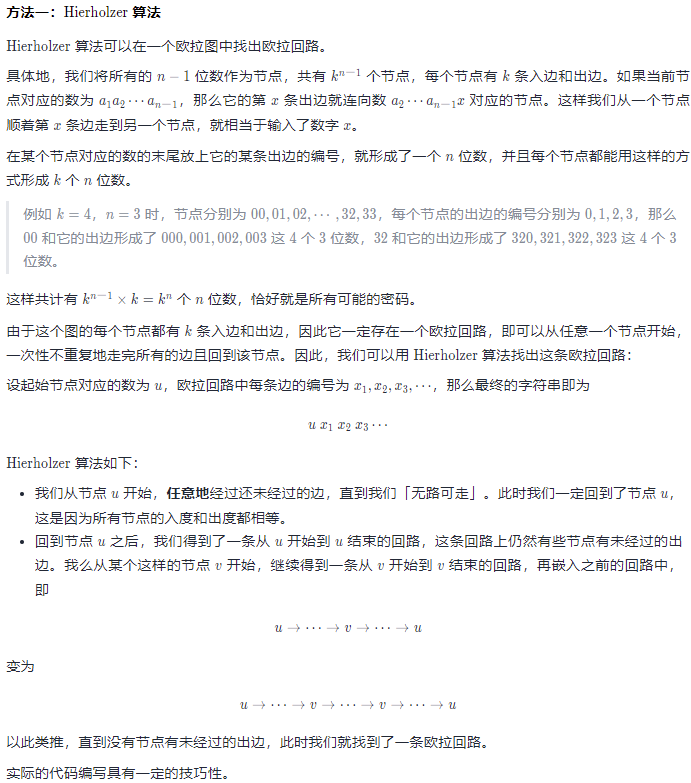
\includegraphics[width=.9\linewidth]{./pic/crackingSafe.png}

由于这个图的每个节点都有 kk 条入边和出边,因此它一定存在一个欧拉回路,即可以从任意一个节点开始,一次性不重复地走完所有的边且回到该节点。因此,我们可以用 \text{Hierholzer}Hierholzer 算法找出这条欧拉回路:
​
我们从节点 uu 开始,任意地经过还未经过的边,直到我们「无路可走」。此时我们一定回到了节点 uu,这是因为所有节点的入度和出度都相等。

回到节点 uu 之后,我们得到了一条从 uu 开始到 uu 结束的回路,这条回路上仍然有些节点有未经过的出边。我么从某个这样的节点 vv 开始,继续得到一条从 vv 开始到 vv 结束的回路,再嵌入之前的回路中,即

u→⋯→v→⋯→u

变为

u→⋯→v→⋯→v→⋯→u

\begin{minted}[fontsize=\scriptsize,linenos=false]{csharp}
Set<Integer> seen = new HashSet<Integer>();
StringBuffer ans = new StringBuffer();
int highest;
int k;
public String crackSafe(int n, int k) {
    highest = (int) Math.pow(10, n - 1);
    this.k = k;
    dfs(0);
    for (int i = 1; i < n; i++) 
        ans.append('0');
    return ans.toString();
}
public void dfs(int node) {
    for (int x = 0; x < k; ++x) {
        int nei = node * 10 + x;
        if (!seen.contains(nei)) {
            seen.add(nei);
            dfs(nei % highest);
            ans.append(x); // 这里dfs之后才添加的顺序狠重要
        }
    }
}
\end{minted}
\item 解题思路与分析
\label{sec-1-5-1-2}

密码共有n位,每一个位可以有k个数字,总共不同的密码总数就有k的n次方个。思路是先从n位都是0的密码开始,取出钥匙串的最后 n-1 个数字,然后在后面依次添加其他数字,用一个 HashSet 来记录所有遍历过的密码,这样如果不在集合中,说明是一个新密码,而生成这个新密码也只是多加了一个数字,能保证钥匙串最短,这是一种贪婪的解法,相当的巧妙

\begin{minted}[fontsize=\scriptsize,linenos=false]{csharp}
public String crackSafe(int n, int k) {
    int N = (int)Math.pow(k, n); // 第个位有k种取值,总共有k^n种不同的状态
    String s = "0".repeat(n);
    Set<String> ss = new HashSet<>(List.of(s.toString()));
    for (int i = 0; i < N; i++) {
        String pre = s.substring(s.length() - (n-1));
        // for (int j = 0; j < k; j++) { // 这里需要倒回来
        for (int j = k-1; j >= 0; j--) { 
            String cur = pre + String.valueOf(j);
            if (!ss.contains(cur)) {
                ss.add(cur);
                s += "" + j;
                break;
            }
        }
    }
    return s;
}
\end{minted}

其实在初看Hierholzer算法时,很容易产生一种想法,就是我只需要从一个节点遍历,每次把它经历的边加入到结果字符串中,当回到初始点时就完成一圈,但是这样实现的话有个明显的问题,就是每个节点都有自环,如果你遍历到某个节点时,直接跳过了自环,去了其他节点,那就失去了回来的机会(想想回家的时候虽然你可以绕小路,也可以走大路,但只要你走大路到家了,就不可能再回到学校从小路回家)。实际上不只是自环,还有可能有其他边没循环到,因为回到自身路径过多,很多边都可能没有利用。

而官方题解中的dfs巧妙的解决了这个问题,实际上它不只是沿着边走,而是把每一个边的组合都遍历到,并且在遍历之后才将有用的节点嵌套到字符串中。在dfs中,每次循环时,并不是直接将该边加入到字符串中,而是在循环之后,实际上可以想成是用了一个栈,反序的将合法的序列弹出了(dfs中的每次循环都会探索一个节点能到达的结尾在哪里,并且因为记录了每一条删除的边,所以其并不会走之前走过的路,找到结尾后回溯到还有边可走的点,继续向下走,而在该点所有可行边都已回溯完毕后,才到他自己,所以其实所有边都已经到达,并且顺序是逆序)。所以在主函数中,在得到整个序列后,才将初始的节点放入字符串末尾(如果正序的话,你应该将它放到字符串的开头)。

\item 解题思路与分析: 递归写法
\label{sec-1-5-1-3}

来看同一种解法的递归写法,思路和迭代的写法一模一样,写法略有不同而已

\begin{minted}[fontsize=\scriptsize,linenos=false]{csharp}
public String crackSafe(int n, int k) {
    N = (int)Math.pow(k, n); // 第个位有k种取值,总共有k^n种不同的状态
    s = "0".repeat(n);
    Set<String> ss = new HashSet<>(List.of(s.toString()));
    dfs(ss, n, k);
    return s;
}
String s;
int N;
void dfs(Set<String> ss, int n, int k) {
    if (ss.size() == N) return; 
    String pre = s.substring(s.length() - (n-1));
    for (int i = k-1; i >= 0; i--) {
        String cur = pre + i;
        if (ss.contains(cur)) continue;
        s += "" + i;
        ss.add(cur);
        dfs(ss, n, k);
    }
}
\end{minted}
\end{enumerate}
\subsection{332. Reconstruct Itinerary - Medium 欧拉回路 Hierholzer 算法}
\label{sec-1-5-2}
You are given a list of airline tickets where tickets[i] = [fromi, toi] represent the departure and the arrival airports of one flight. Reconstruct the itinerary in order and return it.

All of the tickets belong to a man who departs from "JFK", thus, the itinerary must begin with "JFK". If there are multiple valid itineraries, you should return the itinerary that has the smallest lexical order when read as a single string.

For example, the itinerary ["JFK", "LGA"] has a smaller lexical order than ["JFK", "LGB"].
You may assume all tickets form at least one valid itinerary. You must use all the tickets once and only once.
\begin{enumerate}
\item 解题思路与分析
\label{sec-1-5-2-1}

我们化简本题题意:给定一个 nn 个点 mm 条边的图,要求从指定的顶点出发,经过所有的边恰好一次(可以理解为给定起点的「一笔画」问题),使得路径的字典序最小。

\begin{itemize}
\item 这种「一笔画」问题与欧拉图或者半欧拉图有着紧密的联系,下面给出定义:
\begin{itemize}
\item 通过图中所有边恰好一次且行遍所有顶点的通路称为 \textbf{欧拉通路} 。
\item 通过图中所有边恰好一次且行遍所有顶点的回路称为 \textbf{欧拉回路} 。
\item 具有欧拉回路的无向图称为 \textbf{欧拉图} 。
\item 具有欧拉通路但不具有欧拉回路的无向图称为 \textbf{半欧拉图} 。
\end{itemize}
\end{itemize}

因为本题保证至少存在一种合理的路径,也就告诉了我们,这张图是一个欧拉图或者半欧拉图。我们只需要输出这条欧拉通路的路径即可。

\begin{itemize}
\item 如果没有保证至少存在一种合理的路径,我们需要判别这张图是否是欧拉图或者半欧拉图,具体地:
\begin{itemize}
\item 对于无向图 G,G 是欧拉图当且仅当 G 是连通的且没有奇度顶点。
\item 对于无向图 G,G 是半欧拉图当且仅当 G 是连通的且 G 中恰有 2 个奇度顶点。
\item 对于有向图 G,G 是欧拉图当且仅当 G 的所有顶点属于同一个强连通分量且每个顶点的入度和出度相同。
\item 对于有向图 G,G 是半欧拉图当且仅当 G 的所有顶点属于同一个强连通分量且
\begin{itemize}
\item 恰有一个顶点的出度与入度差为 1;
\item 恰有一个顶点的入度与出度差为 1;
\item 所有其他顶点的入度和出度相同。
\end{itemize}
\end{itemize}
\end{itemize}
\item 解题思路与分析: Hierholzer 算法
\label{sec-1-5-2-2}
\begin{itemize}
\item Hierholzer 算法用于在连通图中寻找欧拉路径,其流程如下:
\begin{itemize}
\item 从起点出发,进行深度优先搜索。
\item 每次沿着某条边从某个顶点移动到另外一个顶点的时候,都需要删除这条边。
\item 如果没有可移动的路径,则将所在节点加入到栈中,并返回。
\end{itemize}
\end{itemize}

当我们顺序地考虑该问题时,我们也许很难解决该问题,因为我们无法判断当前节点的哪一个分支是「死胡同」分支。

不妨倒过来思考。我们注意到只有那个入度与出度差为 11 的节点会导致死胡同。而该节点必然是最后一个遍历到的节点。我们可以改变入栈的规则,当我们遍历完一个节点所连的所有节点后,我们才将该节点入栈(即逆序入栈)。

对于当前节点而言,从它的每一个非「死胡同」分支出发进行深度优先搜索,都将会搜回到当前节点。而从它的「死胡同」分支出发进行深度优先搜索将不会搜回到当前节点。也就是说当前节点的死胡同分支将会优先于其他非「死胡同」分支入栈。

这样就能保证我们可以「一笔画」地走完所有边,最终的栈中逆序地保存了「一笔画」的结果。我们只要将栈中的内容反转,即可得到答案。

\begin{minted}[fontsize=\scriptsize,linenos=false]{csharp}
public List<String> findItinerary(List<List<String>> tickets) {
    for (List<String> t : tickets) 
        m.computeIfAbsent(t.get(0), z -> new PriorityQueue<>()).offer(t.get(1));
    List<String> ans = new ArrayList<>();
    dfs("JFK", ans);
    Collections.reverse(ans);
    return ans;
}
Map<String, PriorityQueue<String>> m = new HashMap<>(); // PriorityQueue已经默认是最小字典序,免去了排序的操作
void dfs(String s, List<String> l) {
    Queue<String> next = m.get(s);
    while (next != null && next.size() > 0)
        dfs(next.poll(), l);
    l.add(s);
}
\end{minted}
\item 解题思路与分析: Hierholzer 算法,同上,但用LinkedList可以从头插入
\label{sec-1-5-2-3}

Greedy DFS, building the route backwards when retreating.

这题其实和我之前用 DFS 处理 topological sort 的代码非常像,主要区别在于存 graph 的方式不同,这里是一个 String 直接连着对应的 next nodes,而且形式是 min heap:

\begin{itemize}
\item 原题给的是 edges,所以图是自己用 hashmap 建的。
\begin{itemize}
\item min heap 可以自动保证先访问 lexicographical order 较小的;
\item 同时 poll 出来的 node 自动删除,免去了用 List 的话要先 collections.sort 再 remove 的麻烦。
\item 这种以 “edge” 为重心的算法多靠 heap,比如 dijkstra.
\end{itemize}
\end{itemize}

Hierholzer算法的精髓是当每次访问一条边的时候,删除这条边,当遍历完一个节点所连的所有节点后,才将该节点入栈,最后将栈中的节点反转,即可得到欧拉路径

\begin{minted}[fontsize=\scriptsize,linenos=false]{csharp}
public List<String> findItinerary(String[][] tickets) {
    LinkedList<String> ans = new LinkedList<>();
    for (String[] t : tickets)
        map.computeIfAbsent(t.get(0), z -> new ArrayList<>()).offer(t.get(1));
    dfs("JFK", ans);
    return new ArrayList<String>(ans); // LinkedList最后需要转换成ArrayList
}
HashMap<String, PriorityQueue<String>> map = new HashMap<>();
void dfs(String airport, LinkedList<String> list) {
    while (map.containsKey(airport) && !map.get(airport).isEmpty())
        dfs(map.get(airport).poll(), l);
    list.offerFirst(airport); // LinkedList可以这么写
}
\end{minted}
\item 解题思路与分析: Fleury算法: leetcode还有一道割点割边的题,找出来 todo
\label{sec-1-5-2-4}
\begin{itemize}
\item 一些概念:
\begin{itemize}
\item 割点: 在一个无向图中,如果有一个顶点集合,删除这个顶点集合以及这个集合中所有顶点相关联的边以后,图的连通分量增多,就称这个点集为割点集合,如果某个割点集合只含有一个顶点 X(也即\{X\}是一个割点集合),那么X称为一个割点
\item 割边: 在一个无向图中,如果有一个边集合,删除这个边集合以后,图的连通分量增多,就称这个边集为割边集合,如果某个割边集合只含有一条边 X(也即\{X\}是一个边集合),那么X称为一个割边,也叫做桥
\end{itemize}

\item 步骤
\begin{itemize}
\item 1.如果要找欧拉回路,可以从任意点开始,如果要找欧拉路径,需要从有着奇数度的两个及顶点中的一个开始,如果有奇数度顶点的话
\item 2.选择当前点相连的边,确保删除该边,不会将欧拉图分成两个不同的联通分量
\item 3.将该边加入到路径中,并将该边从欧拉图中删除,如果当前的选择有一个桥与非桥的边时候,优先选非桥的边,不到万不得已,不选桥
\item 4.持续该过程直到路径收集完成
\end{itemize}

\item 分析: 上面的步骤中,选桥边与非桥边的时候,如何判断当前的边是否是桥,这个过程很关键,大体的思路是:
\begin{itemize}
\item 从当前节点u出发,计数,哪些顶点可以通过u可达,直接可达和间接可达均可以,记为cnt1
\item 移除掉u-v这条边
\item 从当前节点v出发,,哪些顶点可以通过v可达,直接可达和间接可达均可以,记为cnt2
\item 恢复u-v这条边
\item 返回cnt1与cnt2的大小,如果cnt2要比cnt1小,说明移除u-v这条边,从v可达的顶点数量减少,产生了额外的联通分量,此时返回falase,说明这条边是桥,反之返回true

\begin{minted}[fontsize=\scriptsize,linenos=false]{csharp}
public List<String> findItinerary(List<List<String>> tickets) { // 这个算法还比较陌生
    for (List<String> t : tickets) 
        adj.computeIfAbsent(t.get(0), z -> new ArrayList<>()).add(t.get(1));
    for (List<String> values : adj.values()) Collections.sort(values);
    String u = "JFK";
    ans.add(u);
    fleuryProcess(u);
    return ans;
}
Map<String, List<String>> adj = new HashMap<>();
List<String> ans = new ArrayList<>();
private void fleuryProcess(String u) {
    if (!adj.containsKey(u)) return ;
    for (int i = 0; i < adj.get(u).size(); i++) {
        String v = adj.get(u).get(i);
        if (isValidNextEdge(u, v)) {
            ans.add(v);
            adj.get(u).remove(v);
            fleuryProcess(v);
        }
    }
}
private boolean isValidNextEdge(String u, String v) { // 判断是否是割边:
    if (adj.get(u).size() == 1) return true;
    // boolean[] visited = new boolean[adj.get(u).size()];
    Map<String, Boolean> vis = new HashMap<>(); // vis: visited
    int cnt1 = dfs(u, vis);
    adj.get(u).remove(v);
    vis.clear(); // vis = new HashMap<>();
    int cnt2 = dfs(v, vis);
    adj.get(u).add(0, v);
    return cnt1 <= cnt2; // 如果cnt2要比cnt1小,说明移除u-v这条边,从v可达的顶点数量减少,产生了额外的联通分量,此时返回 falase, 说明这条边是桥; 反之返回 true 
}
private int dfs(String u, Map<String, Boolean> vis) {
    vis.put(u, true);
    int cnt = 1;
    if (adj.containsKey(u)) 
        for (String v : adj.get(u)) 
            if (vis.get(v) == null || (vis.get(v) != null && !vis.get(v))) 
                cnt += dfs(v, vis);
    return cnt;
}
\end{minted}
\end{itemize}
\end{itemize}
\end{enumerate}
\subsection{2097. Valid Arrangement of Pairs - Hard 欧拉回路}
\label{sec-1-5-3}
You are given a 0-indexed 2D integer array pairs where pairs[i] = [starti, endi]. An arrangement of pairs is valid if for every index i where 1 <= i < pairs.length, we have endi-1 == starti.

Return any valid arrangement of pairs.

Note: The inputs will be generated such that there exists a valid arrangement of pairs.
\begin{enumerate}
\item 解题思路与分析
\label{sec-1-5-3-1}
\begin{minted}[fontsize=\scriptsize,linenos=false]{csharp}
// One thing different is that we need to find the start point. it is obvious that if indegree is larger than 0, that is the start point.
public int[][] validArrangement(int[][] pairs) { 
    Map<Integer, Integer> ins = new HashMap<>();
    for (int [] p : pairs) {
        adj.computeIfAbsent(p[0], z -> new ArrayList<>()).add(p[1]);
        ins.put(p[0], ins.getOrDefault(p[0], 0) + 1);
        ins.put(p[1], ins.getOrDefault(p[1], 0) - 1);
    }
    int bgn = -1;
    for (Integer key : ins.keySet()) 
        if (ins.get(key) > 0) {
            bgn = key;
            break;
        }
    if (bgn == -1) bgn = pairs[0][0]; // 如果没有,就可以随便从某一个点开始?
    dfs(bgn);
    int n = pairs.length;
    int [][] ans = new int [n][];
    for (int i = n-1; i >= 0; i--) // 所以这里添加答案,也需要反序回正
        ans[n-1-i] = ll.get(i);
    return ans;
}
Map<Integer, List<Integer>> adj = new HashMap<>();
List<int []> ll = new ArrayList<>();
void dfs(int node) {
    while (adj.get(node) != null && adj.get(node).size() > 0) {
        List<Integer> nextNodesCandi = adj.get(node);
        int next = nextNodesCandi.get(nextNodesCandi.size()-1); // 从后往前遍历,方便从后往前删除已经遍历过的节点
        adj.get(node).remove(nextNodesCandi.size()-1);
        dfs(next);
        ll.add(new int [] {node, next}); // 这里的顺序是倒着加的,dfs完接下来的答案、之后再加的
    }
}
\end{minted}
\item 解题思路与分析: todo: 这个答案没有看懂
\label{sec-1-5-3-2}
\begin{minted}[fontsize=\scriptsize,linenos=false]{csharp}
// In a word, this solution is to first determine whether the target is an Euler circuit or an Euler path, then solve it.
public int[][] validArrangement(int[][] pairs) {
    int n = pairs.length;
    Map<Integer, Integer> outdegree = new HashMap<>();
    Map<Integer, Deque<Integer>> out = new HashMap<>();
    for (int[] pair : pairs) {
        outdegree.put(pair[0], outdegree.getOrDefault(pair[0], 0) + 1);
        outdegree.put(pair[1], outdegree.getOrDefault(pair[1], 0) - 1);
    }
    int[][] ans = new int[n][2];
    for (int i = 0; i < n; i++) 
        Arrays.fill(ans[i], -1);
    for (Map.Entry<Integer, Integer> en : map.entrySet()) { // 试图寻找起始和结束的位置
        if (en.getValue() == 1) ans[0][0] = en.getKey();
        if (en.getValue() == -1) ans[n-1][1] = en.getKey();
    }
    if (ans[0][0] == -1) { // 这里为什么就可以从第一个往后搜、从两边往中间搜呢?
        ans[0][0] = pairs[0][0];
        ans[n-1][1] = pairs[0][0];
    }
    for (int[] p : pairs) {
        out.computeIfAbsent(p[0], z -> new ArrayDeque<>()).offerLast(p[1]);
        // out.computeIfAbsent(p[0], k -> new ArrayDeque<>());
        out.computeIfAbsent(p[1], k -> new ArrayDeque<>()); // 需要加上
        // out.get(p[0]).offerLast(p[1]);
    }
    int i = 0, j = n-1;
    while (i < j) { // 没看明白这中间在是做什么???
        int from = ans[i][0];
        Deque<Integer> toList = out.get(from); // 这里是个栈, 上面如果不加上,这里会是null
        if (toList.size() == 0) {
            i--;
            ans[j][0] = ans[i][0];
            j--;
            ans[j][1] = ans[j + 1][0];
        } else {
            ans[i++][1] = toList.pollLast();
            // ans[i++][1] = toList.removeLast();
            ans[i][0] = ans[i - 1][1];
        }
    }
    return ans;
}
\end{minted}
\end{enumerate}

\subsection{1591. Strange Printer II - Hard}
\label{sec-1-5-4}
There is a strange printer with the following two special requirements:

On each turn, the printer will print a solid rectangular pattern of a single color on the grid. This will cover up the existing colors in the rectangle.
Once the printer has used a color for the above operation, the same color cannot be used again.
You are given a m x n matrix targetGrid, where targetGrid[row][col] is the color in the position (row, col) of the grid.

Return true if it is possible to print the matrix targetGrid, otherwise, return false.

\begin{enumerate}
\item 解题思路与分析: 邻接有向图 + 拓扑排序
\label{sec-1-5-4-1}

这道题可以认为是在研究:是否有一种颜色序列,按照这个序列进行染色,最终矩阵就会呈现输入的状态。

矩形上的某一个像素点,可能会先后经历多次染色。比如先染红,再染绿,再染黄,最后染蓝,最后呈现出的就是蓝色。

我们知道这个像素现在是蓝色;

而它在红色/绿色/黄色矩形范围内,说明这个像素曾经红过/绿过/黄过。

此时我们可以提炼出信息:假定先染的优先于后染的,那么红色优于蓝色,绿色优于蓝色,黄色优于蓝色。

(红绿黄之间的顺序未定)。

题中指出,颜色最多有 6060 种,我们可以建立一个有向图,图中的结点就是这 6060 个颜色 1$\sim$ 601∼60 。

按照刚才的方法找出所有的有向边,进行拓扑排序即可判断出结果。

\begin{minted}[fontsize=\scriptsize,linenos=false]{csharp}
public boolean isPrintable(int[][] a) { 
    int m = a.length, n = a[0].length, max = Math.max(m, n);
    for (int i = 0; i < m; i++)
        max = Math.max(max, Arrays.stream(a[i]).max().getAsInt());
    int N = max + 1;
    int [] up = new int [N], down = new int [N], left = new int [N], right = new int [N];
    Arrays.fill(up, m);
    Arrays.fill(left, n);
    Arrays.fill(down, -1);
    Arrays.fill(right, -1);
    for (int i = 0; i < m; i++) // 界定每一种着色的上下左右边界,以便接下来排序
        for (int j = 0; j < n; j++) {
            int k = a[i][j];
            up[k] = Math.min(up[k], i);
            down[k] = Math.max(down[k], i);
            left[k] = Math.min(left[k], j);
            right[k] = Math.max(right[k], j);
        }
    // 根据每种着色的界定范围,建立拓扑排序:这后半部分还有点儿不熟练
    // 当前位置颜色 cur 在某个矩阵 k 中但是不为矩阵 k 的颜色时,建立从 k 到 cur 的边,cur 可以存在于多个矩阵中
    boolean [][] nei = new boolean [N][N];  // neighbours
    List<Integer>[] adj = new ArrayList[N]; // 邻接有向图:按照染色的先后顺序
    int [] ins = new int [N];
    for (int i = 0; i < N; i++) adj[i] = new ArrayList<>();
    for (int i = 0; i < m; i++)
        for (int j = 0; j < n; j++) {
            int cur = a[i][j]; // 当前格的最终打印着色
            for (int k = 1; k < N; k++) { // 遍历所有的着色:暴搜当前着色cur是否会在某种着色k之后染色
                if (k == cur) continue;
                if (i >= up[k] && i <= down[k] && j >= left[k] && j <= right[k])  // 现着色cur完全处于先前染色k的内部,所以cur是后着色
                    // if (!nei[cur][k]) { // BUG: 是有向图:这里顺序很重要,先染色 是否 与后染色相连/相前后
                    if (!nei[k][cur]) {    // k 先染后, cur 后染色
                        adj[k].add(cur);
                        ins[cur]++;
                        nei[k][cur] = true;
                    }
            }
        }
    List<Integer> l = new ArrayList<>();
    while (true) { // 寻找入度为 0 的颜色点,减小该点连结的点的入度,直到所有点的入度都为 0
        int i;
        for (i = 1; i < N; i++) 
            if (ins[i] == 0) {
                l.add(i);
                for (int v : adj[i]) ins[v]--;
                ins[i] = -1;
                break;
            }
        if (i == N) break;
    }
    return l.size() == max; // 按照拓扑排序,这所有的染色都可以有序地染出来,那么合法
}
\end{minted}
\item 解题思路与分析: topological sort
\label{sec-1-5-4-2}
\begin{minted}[fontsize=\scriptsize,linenos=false]{csharp}
public boolean isPrintable(int[][] a) { 
    int m = a.length, n = a[0].length;
    Set<Integer> col = new HashSet<>();
    for (int i = 0; i < m; i++) 
        for (int j = 0; j < n; j++)
            col.add(a[i][j]);
    for (Integer c : col) {
        int fi = -1, fj = Integer.MAX_VALUE, li = -1, lj = -1;  // f: first, f row, f col, l: last, l row, l col
        for (int i = 0; i < m; i++)
            for (int j = 0; j < n; j++)
                if (a[i][j] == c) {
                    if (fi == -1) fi = i; // 只记最早出现的第一次
                    fj = Math.min(fj, j);
                    li = i;
                    lj = Math.max(lj, j);
                }
        for (int i = fi; i <= li; i++) 
            for (int j = fj; j <= lj; j++) 
                if (a[i][j] != c) // a[i][j]是会在当前染色c之后染色的
                    adj.computeIfAbsent(c, z -> new HashSet<>()).add(a[i][j]);
    }
    Set<Integer> vis = new HashSet<>(); // visiting: 只保证先染的着色不会在后染的着色里再次出现
    for (Integer c : col) 
        if (!topologicalSort(vis, c)) return false;
    return true;
}
Map<Integer, Set<Integer>> adj = new HashMap<>(); // 在key之后染色的着色集合
private boolean topologicalSort(Set<Integer> vis, int c) { // 这种写法好陌生
    if (vis.contains(c)) return false;
    vis.add(c);
    for (Integer nei : adj.getOrDefault(c, Collections.emptySet()))
        if (!topologicalSort(vis, nei)) return false;
    vis.remove(c);
    return true;
}
\end{minted}
\end{enumerate}


\section{双端队列BFS}
\label{sec-1-6}
\subsection{1368. Minimum Cost to Make at Least One Valid Path in a Grid - Hard}
\label{sec-1-6-1}
Given a m x n grid. Each cell of the grid has a sign pointing to the next cell you should visit if you are currently in this cell. The sign of grid[i][j] can be:
1 which means go to the cell to the right. (i.e go from grid[i][j] to grid[i][j + 1])
2 which means go to the cell to the left. (i.e go from grid[i][j] to grid[i][j - 1])
3 which means go to the lower cell. (i.e go from grid[i][j] to grid[i + 1][j])
4 which means go to the upper cell. (i.e go from grid[i][j] to grid[i - 1][j])
Notice that there could be some invalid signs on the cells of the grid which points outside the grid.

You will initially start at the upper left cell (0,0). A valid path in the grid is a path which starts from the upper left cell (0,0) and ends at the bottom-right cell (m - 1, n - 1) following the signs on the grid. The valid path doesn't have to be the shortest.

You can modify the sign on a cell with cost = 1. You can modify the sign on a cell one time only.

Return the minimum cost to make the grid have at least one valid path.
\begin{enumerate}
\item 解题思路与分析: 0-1广度优先搜索(最优解法)
\label{sec-1-6-1-1}

这道题其实是个经典的双端队列BFS。将每个格子看成是图的顶点,相邻格子是有边相连接的。如果从顶点(x, y)到(u, v)的实际方向和矩阵在(x, y)所表示的方向相同,则令这条边的边权为0,否则令其边权为1。原题相当于在问,在此图中,从起点到终点的最短路长度是多少。由于边权只有0和1两种,所以可以用双端队列BFS来做。每次拓展的时候,如果是沿着边权0的边走的,则插入队头,否则插入队尾。从队列里取元素的时候永远都从队头取。然后用堆优化的Dijkstra算法模板来写即可。时空复杂度O(mn)。

0-1 广度优先搜索的实现其实与 Dijkstra 算法非常相似。在 Dijkstra 算法中,我们用优先队列保证了距离的单调递增性。而在 0-1 广度优先搜索中,实际上任意时刻队列中的节点与源点的距离均为 dd 或 d + 1d+1(其中 dd 为某一非负整数),并且所有与源点距离为 dd 的节点都出现在队首附近,所有与源点距离为 d + 1d+1 的节点都出现在队尾附近。因此,我们只要使用双端队列,对于边权为 00 和 11 的两种情况分别将对应节点添加至队首和队尾,就保证了距离的单调递增性。

\begin{minted}[fontsize=\scriptsize,linenos=false]{csharp}
public int minCost(int[][] g) {
    int m = g.length, n = g[0].length;
    int [][] d = new int [m][n]; // dist to [0, 0]
    for (int i = 0; i < m; i++) 
        Arrays.fill(d[i], Integer.MAX_VALUE);
    d[0][0] = 0;
    int [][] dirs = {{0, 0}, {0, 1}, {0, -1}, {1, 0}, {-1, 0}}; // [0, 1, 2, 3, 4]
    boolean [][] vis = new boolean [m][n];
    ArrayDeque<Integer> q = new ArrayDeque<>();
    q.offerFirst(0);
    while (!q.isEmpty()) {
        int idx = q.pollFirst();
        int i = idx / n, j = idx % n;
        if (vis[i][j]) continue;
        if (i == m-1 && j == n-1) return d[i][j];
        vis[i][j] = true;
        for (int k = 1; k < 5; k++) {
            int x = i + dirs[k][0], y = j + dirs[k][1];
            if (x < 0 || x >= m || y < 0 || y >= n) continue;
            int cost = k == g[i][j] ? 0 : 1;
            if (!vis[x][y] && d[x][y] > d[i][j] + cost) {
                d[x][y] = d[i][j] + cost;
                if (cost == 0) q.offerFirst(x * n + y);
                else q.offerLast(x * n + y);
            }
        }
    }
    return -1;
}
\end{minted}
\item 解题思路与分析: 最短路径问题总结 BFS
\label{sec-1-6-1-2}
\begin{enumerate}
\item 题目分析
\label{sec-1-6-1-2-1}
\begin{itemize}
\item 虽然题目的描述中写了有效路径不需要是最短路径,但其实这道题目还是一个最短路径问题,只不过要求的最短距离并不是在网格中行走的距离,而是改变方向的次数。
\item 所谓最短路径问题,就是对于图 G(V,E)G(V,E),寻找从 u$\in$ Vu∈V 到 v$\in$ Vv∈V 的最短距离。最短路径的算法有很多,包括 Dijkstra,Floyd,Bellman-Ford,SPFA 等。
\end{itemize}

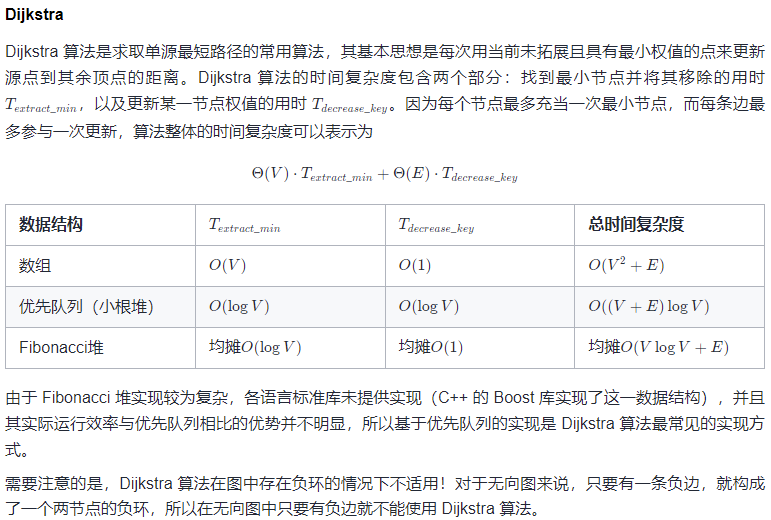
\includegraphics[width=.9\linewidth]{./pic/1368.png}

对于 BFS,相信大家一定都很熟悉了。与 DFS 相比,BFS 的特点是按层遍历,从而可以保证首先找到最优解(最少步数、最小深度)。从这个意义上讲,BFS 解决的其实也是最短路径问题。这一问题对应的图 GG 包含的所有顶点即为状态空间,而每一个可能的状态转移都代表了一条边。

比如,在经典的迷宫问题中,每一个状态 (x,y)(x,y) 代表了一个顶点,而一个无障碍格子与其相邻的无障碍格子之间则存在一条无向边。

那么,这个图 GG 和一般的图相比,有什么特点呢?

关键就在于边的权值。在 BFS 问题中,所有边的权值均为 1!因为我们每一次从一个状态转移到一个新的状态,就多走了一步。正因为边权值均为 1,我们用一个队列记录所有状态,前面的状态对应的总权值一定小于后面的状态,所以我们就可以在 O(1)O(1) 的时间内实现找到最小节点并将其移除的操作(只要取队头,然后出队就可以了),从而寻找最短路径的时间复杂度就减小到了 O(V+E)O(V+E)。

但普通的 BFS 算法,在本题中并不适用,因为存在权值为 0 的边!如果从一个格子到另一个格子,不需要修改格子上的标记,那么这一步移动的权值就为 0。如果我们还沿用普通 BFS 的做法,就无法保证队头元素一定是当前具有最小权值的节点。

怎么办呢?简单粗暴的做法是:允许多次扩展同一个点。只要当前边能够更新节点的权值,就将节点再次入队。

\begin{minted}[fontsize=\scriptsize,linenos=false]{csharp}
public int minCost(int[][] g) {
    int [][] dirs = {{0, 0}, {0, 1}, {0, -1}, {1, 0}, {-1, 0}}; 
    int m = g.length, n = g[0].length;
    int [][] d = new int [m][n]; // dist to [0, 0]
    for (int i = 0; i < m; i++) 
        Arrays.fill(d[i], Integer.MAX_VALUE);
    d[0][0] = 0;
    Queue<int []> q = new LinkedList<>();
    q.offer(new int [] {0, 0});
    while (!q.isEmpty()) {
        int [] cur = q.poll();
        int i = cur[0], j = cur[1];
        for (int k = 1; k < 5; k++) {
            int x = i + dirs[k][0], y = j + dirs[k][1];
            if (x < 0 || x >= m || y < 0 || y >= n) continue;
            int newDist = d[i][j] + (k == g[i][j] ? 0 : 1);
            if (newDist < d[x][y]) {
                d[x][y] = newDist;
                q.offer(new int [] {x, y});
            }
        }
    }
    return d[m-1][n-1];
}
\end{minted}
\end{enumerate}
\item 解题思路与分析: SPFA
\label{sec-1-6-1-3}
如果一个节点已经在队列中,其实就没有必要将其再次入队了。这是 SPFA 算法的基本思想。可以看到,与上面的BFS 方法相比,就是增加了一个 in 数组来判断当前节点是否已经在队列中。

SPFA 算法是一个十分依赖于数据的算法。在特定的数据下,SPFA 会退化为 Bellman-Ford,时间复杂度为 O(V$\cdot$ E)O(V⋅E)。一般的编程竞赛中,涉及到最短路径的题目,都会有专门卡SPFA的数据,所以一般情况下还是使用 Dijkstra 算法。本题的测试数据相对较弱,BFS 和 SPFA 都可以顺利通过,甚至 SPFA 的运行时间还要长于 BFS(修改 in 数组状态带来了额外的开销)。

SPFA 的好处是可以判断负环。我们可以用一个数组记录每个顶点的入队次数,如果有顶点的入队次数超过了 VV 次,则代表图中存在负环。

\begin{minted}[fontsize=\scriptsize,linenos=false]{csharp}
public int minCost(int[][] g) {
    int [][] dirs = {{0, 0}, {0, 1}, {0, -1}, {1, 0}, {-1, 0}}; 
    int m = g.length, n = g[0].length;
    int [][] d = new int [m][n]; 
    for (int i = 0; i < m; i++) 
        Arrays.fill(d[i], Integer.MAX_VALUE);
    d[0][0] = 0;
    boolean [][] in = new boolean [m][n];
    Queue<int []> q = new LinkedList<>();
    q.offer(new int [] {0, 0});
    in[0][0] = true;
    while (!q.isEmpty()) {
        int [] cur = q.poll();
        int i = cur[0], j = cur[1];
        in[i][j] = false;
        for (int k = 1; k < 5; k++) {
            int x = i + dirs[k][0], y = j + dirs[k][1];
            if (x < 0 || x >= m || y < 0 || y >= n) continue;
            int newDist = d[i][j] + (k == g[i][j] ? 0 : 1);
            if (newDist < d[x][y]) {
                d[x][y] = newDist;
                if (!in[x][y]) {
                    q.offer(new int [] {x, y});
                    in[x][y] = true;
                }
            }
        }
    }
    return d[m-1][n-1];
}
\end{minted}
\item 解题思路与分析
\label{sec-1-6-1-4}
\end{enumerate}

\subsection{126. Word Ladder II - Hard BFS}
\label{sec-1-6-2}
A transformation sequence from word beginWord to word endWord using a dictionary wordList is a sequence of words beginWord -> s1 -> s2 -> \ldots{} -> sk such that:

Every adjacent pair of words differs by a single letter.
Every si for 1 <= i <= k is in wordList. Note that beginWord does not need to be in wordList.
sk == endWord
Given two words, beginWord and endWord, and a dictionary wordList, return all the shortest transformation sequences from beginWord to endWord, or an empty list if no such sequence exists. Each sequence should be returned as a list of the words [beginWord, s1, s2, \ldots{}, sk].
\begin{enumerate}
\item 解题思路与分析: 广度优先搜索
\label{sec-1-6-2-1}
\begin{itemize}
\item 官方题解:\url{https://leetcode-cn.com/problems/word-ladder-ii/solution/dan-ci-jie-long-ii-by-leetcode-solution/}

\begin{minted}[fontsize=\scriptsize,linenos=false]{csharp}
public List<List<String>> findLadders(String bgn, String end, List<String> list) { 
    Set<String> ss = new HashSet<>(list);
    if (!ss.contains(end)) return ans;
    ss.remove(bgn);
    // BFS: 第 1 步:广度优先遍历建图
    Map<String, Integer> cnt = new HashMap<>(); // 记录扩展出的单词是在第几次扩展的时候得到的,key:单词,value:在广度优先遍历的第几层
    cnt.put(bgn, 0);
    Map<String, List<String>> from = new HashMap<>(); // 记录了单词是从哪些单词扩展而来,key:单词,value:单词列表,这些单词可以变换到 key ,它们是一对多关系
    int step = 1, n = bgn.length();
    boolean found = false;
    Queue<String> q = new LinkedList<>();
    q.offer(bgn);
    while (!q.isEmpty()) {
        for (int size = q.size()-1; size >= 0; size--) {
            String cur = q.poll();
            char [] s = cur.toCharArray();
            for (int i = 0; i < n; i++) {
                char ori = s[i];
                for (char c = 'a'; c <= 'z'; c++) {
                    if (s[i] == c) continue; // 
                    s[i] = c;
                    String next = String.valueOf(s);
                    if (cnt.containsKey(next) && step == cnt.get(next)) //
                        from.get(next).add(cur);                        //
                    if (!ss.contains(next)) continue; // BUG: 还没有想明白,为什么我把这行写前面会少掉答案呢? 
                    ss.remove(next); // 如果从一个单词扩展出来的单词以前遍历过,距离一定更远,为了避免搜索到已经遍历到,且距离更远的单词,需要将它从 dict 中删除
                    q.offer(next);   // 这一层扩展出的单词进入队列
                    from.computeIfAbsent(next, z -> new ArrayList<>()).add(cur); // 记录 next Word 从 cur Word 而来
                    cnt.put(next, step);
                    if (next.equals(end)) found = true;
                }
                s[i] = ori;
            }
        }
        step++;
        if (found) break;
    }
    // 第 2 步:深度优先遍历找到所有解,从 end 恢复到 bgn ,所以每次尝试操作 path 列表的头部
    if (found) {
        Deque<String> path = new ArrayDeque<>(); 
        path.add(end);
        dfs(from, path, bgn, end);
    }
    return ans;
}
List<List<String>> ans = new ArrayList<>();
void dfs(Map<String, List<String>> from, Deque<String> path, String end, String cur) {
    if (cur.equals(end)) {
        ans.add(new ArrayList<>(path)); // 这个写法学习一下,第一次见
        return ;
    }
    for (String precursor : from.get(cur)) {
        path.offerFirst(precursor);
        dfs(from, path, end, precursor);
        path.pollFirst();
    }
}
\end{minted}
\end{itemize}
\item 解题思路与分析: 详细通俗的思路分析,多解法: DFS + BFS 双向搜索(two-end BFS)双向BFS搜索
\label{sec-1-6-2-2}
\begin{itemize}
\item \url{https://leetcode-cn.com/problems/word-ladder-ii/solution/xiang-xi-tong-su-de-si-lu-fen-xi-duo-jie-fa-by-3-3/}
\end{itemize}

这个题解和自己最初解法比较接近,需要再好好学习一下
\begin{minted}[fontsize=\scriptsize,linenos=false]{csharp}
 public List<List<String>> findLadders(String beginWord, String endWord, List<String> wordList) {
    List<List<String>> ans = new ArrayList<>();
    if (!wordList.contains(endWord)) return ans;
    // 利用 BFS 得到所有的邻居节点
    HashMap<String, ArrayList<String>> map = new HashMap<>();
    bfs(beginWord, endWord, wordList, map);
    ArrayList<String> temp = new ArrayList<String>();
    // temp 用来保存当前的路径
    temp.add(beginWord);
    findLaddersHelper(beginWord, endWord, map, temp, ans);
    return ans;
}
private void findLaddersHelper(String beginWord, String endWord, HashMap<String, ArrayList<String>> map,
                               ArrayList<String> temp, List<List<String>> ans) {
    if (beginWord.equals(endWord)) {
        ans.add(new ArrayList<String>(temp));
        return;
    }
    // 得到所有的下一个的节点
    ArrayList<String> neighbors = map.getOrDefault(beginWord, new ArrayList<String>());
    for (String neighbor : neighbors) {
        temp.add(neighbor);
        findLaddersHelper(neighbor, endWord, map, temp, ans);
        temp.remove(temp.size() - 1);
    }
}
// 利用递归实现了双向搜索
private void bfs(String beginWord, String endWord, List<String> wordList, HashMap<String, ArrayList<String>> map) {
    Set<String> set1 = new HashSet<String>();
    set1.add(beginWord);
    Set<String> set2 = new HashSet<String>();
    set2.add(endWord);
    Set<String> wordSet = new HashSet<String>(wordList);
    bfsHelper(set1, set2, wordSet, true, map);
}
// direction 为 true 代表向下扩展,false 代表向上扩展
private boolean bfsHelper(Set<String> set1, Set<String> set2, Set<String> wordSet, boolean direction,
                          HashMap<String, ArrayList<String>> map) {
    // set1 为空了,就直接结束
    // 比如下边的例子就会造成 set1 为空
    /*	"hot"
        "dog"
        ["hot","dog"]*/
    if (set1.isEmpty()) return false;
    // set1 的数量多,就反向扩展
    if (set1.size() > set2.size()) 
        return bfsHelper(set2, set1, wordSet, !direction, map);
    // 将已经访问过单词删除
    wordSet.removeAll(set1);
    wordSet.removeAll(set2);
    boolean done = false;
    // 保存新扩展得到的节点
    Set<String> set = new HashSet<String>();
    for (String str : set1) {
        // 遍历每一位
        for (int i = 0; i < str.length(); i++) {
            char[] chars = str.toCharArray();
            // 尝试所有字母
            for (char ch = 'a'; ch <= 'z'; ch++) {
                if(chars[i] == ch) continue;
                chars[i] = ch;
                String word = new String(chars);
                // 根据方向得到 map 的 key 和 val
                String key = direction ? str : word;
                String val = direction ? word : str;
                ArrayList<String> list = map.containsKey(key) ? map.get(key) : new ArrayList<String>();
                // 如果相遇了就保存结果
                if (set2.contains(word)) {
                    done = true;
                    list.add(val);
                    map.put(key, list);
                }
                // 如果还没有相遇,并且新的单词在 word 中,那么就加到 set 中
                if (!done && wordSet.contains(word)) {
                    set.add(word);
                    list.add(val);
                    map.put(key, list);
                }
            }
        }
    }
    // 一般情况下新扩展的元素会多一些,所以我们下次反方向扩展  set2
    return done || bfsHelper(set2, set, wordSet, !direction, map);
}
\end{minted}
\end{enumerate}

\section{环与入度等}
\label{sec-1-7}
\subsection{685. Redundant Connection II - Hard}
\label{sec-1-7-1}
In this problem, a rooted tree is a directed graph such that, there is exactly one node (the root) for which all other nodes are descendants of this node, plus every node has exactly one parent, except for the root node which has no parents.

The given input is a directed graph that started as a rooted tree with n nodes (with distinct values from 1 to n), with one additional directed edge added. The added edge has two different vertices chosen from 1 to n, and was not an edge that already existed.

The resulting graph is given as a 2D-array of edges. Each element of edges is a pair [ui, vi] that represents a directed edge connecting nodes ui and vi, where ui is a parent of child vi.

Return an edge that can be removed so that the resulting graph is a rooted tree of n nodes. If there are multiple answers, return the answer that occurs last in the given 2D-array.
\begin{enumerate}
\item 解题思路与分析
\label{sec-1-7-1-1}
\begin{minted}[fontsize=\scriptsize,linenos=false]{csharp}
// 对于有向图中,如果存在indegree(v) == 2的点,那么要删除的一定是这个点的某条有向边(u -> v)
//    因为题目最后保证是一个rooted tree(every node has exactly one parent),具体看第一段定义;
// 如果不存在indegree(v) == 2的点,那么直接删去最后一个造成环存在的有向边即可。
// 现在存在三种情况:
// (1)有向图中只有环。这种情况就简单将两个节点具有共同根节点的边删去就好。
// (2)有向图中没有环,但有个节点有两个父节点。这种情况就将第二次出现不同父节点的边删去就好。
// (3)有向图中既有环,而且有个节点还有两个父节点。这时就检测当除去第二次出现父节点的边后,剩余边是不是合法的,如果不合法证明应该删掉的是另一个父节点的边。
public int [] findRedundantDirectedConnection(int [][] egs) {
    Set<Integer> p = new HashSet<>();
    Map<Integer, Integer> par = new HashMap<>(); // k,v: v <-- u
    List<int []> candi = new ArrayList<>();
    for (int [] e : egs) {
        int u = e[0], v = e[1];
        p.add(u);
        p.add(v);
        if (!par.containsKey(v)) { // 对于入度为1的右端点边,记在字典里
            par.put(v, u);
            continue;
        }
        candi.add(new int [] {par.get(v), v}); // 第一次出现的边
        candi.add(new int [] {u, v});          // 第二次出现的边,答案是这两者之一
        e[1] = -1; // 先将后出现的第二条边废掉,验证答案
    }
    UnionFind uf = new UnionFind(p.size()); // 总顶点的个数
    for (int [] e : egs) {
        if (e[1] == -1) continue;   // 跳过正在验证是否为的答案后出现的第二条边
        int u = e[0]-1, v = e[1]-1; // uf 0-based
        if (!uf.union(u, v)) { // 在已经废除后出现的第二条边之后,还是出现了环,那么后出现的第二条边不是答案,第一条才是
            if (candi.isEmpty()) return e; // 不存在入度为 2 的点,直接删去最后一条造成环存在的有向边, 即当前边即可
            return candi.get(0);
        }
    }
    return candi.get(1); // 删除第二条边后,所有的存在都合法,那么就返回第二条边
}
class UnionFind {
    int[] parent;
    int[] rank;
    int size;
    public UnionFind(int size) {
        this.size = size;
        parent = new int[size];
        rank = new int[size];
        for (int i = 0; i < size; i++) parent[i] = i;
    }
    public int find(int x) {
        if (parent[x] != x) 
            parent[x] = find(parent[x]);
        return parent[x];
    }
    public boolean union(int x, int y) { 
        int xp = find(x);
        int yp = find(y);
        if (xp == yp) return false; // 已经在同一个强连通分量中
        if (rank[xp] > rank[yp]) 
            parent[yp] = xp;
        else if (rank[xp] < rank[yp]) 
            parent[xp] = yp;
        else {
            parent[yp] = xp;
            rank[xp]++;
        }
        return true;
    }
}
\end{minted}
\end{enumerate}
\section{普通BFS,但state状态狠重要}
\label{sec-1-8}
\subsection{1293. Shortest Path in a Grid with Obstacles Elimination - Hard}
\label{sec-1-8-1}
You are given an m x n integer matrix grid where each cell is either 0 (empty) or 1 (obstacle). You can move up, down, left, or right from and to an empty cell in one step.

Return the minimum number of steps to walk from the upper left corner
(0, 0) to the lower right corner (m - 1, n - 1) given that you can
eliminate at most k obstacles. If it is not possible to find such walk
return -1.
\begin{enumerate}
\item 解题思路与分析
\label{sec-1-8-1-1}
\begin{itemize}
\item 在普通的bfs中,为了避免走重复的路径,我们一般采用visited数组来记录下走过的格子,当路径遇到一个已走过的格子时,便不能再通过该点。但本题略有不同,上面说过,本题存在两种路径,因此visited数组中的状态应该包含3中状态:
\begin{itemize}
\item 0:该位置没有走过
\item 1:该位置被普通路径走过
\item 2:该路径被穿越路径走过
\end{itemize}
\item 对于以上三种状态,
\begin{itemize}
\item 当前格子为非障碍物时,普通路径可以走访问状态为0的格子,走过后,访问状态更新为1
\item 当前格子为非障碍物时,穿越路径可以走访问状态为0的格子,走过后,访问状态更新为2
\item 当前格子为非障碍物时,普通路径可以走访问状态为2的格子,走过后,访问状态更新为1
\item 当前格子为障碍物时,如果还保有穿越次数,并且该格子的访问状态为0时,所有路径可以通过此处,通过后,该路径变为穿越路径,并且当前格子访问状态更新为1(更新为2也无所谓)
\begin{minted}[fontsize=\scriptsize,linenos=false]{csharp}
public int shortestPath(int[][] a, int k) {
    int [][] dirs = {{1, 0}, {-1, 0}, {0, 1}, {0, -1}};
    int m = a.length, n = a[0].length;
    int [][] vis = new int [m][n]; 
    Deque<int []> q = new ArrayDeque<>();
    q.offerLast(new int [] {0, 0, k});
    int cnt = 0;
    while (!q.isEmpty()) {
        for (int z = q.size()-1; z >= 0; z--) {
            int [] cur = q.pollFirst();
            if (cur[0] == m-1 && cur[1] == n-1) return cnt;
            for (int [] d : dirs) {
                int i = cur[0] + d[0], j = cur[1] + d[1];
                if (i >= 0 && i < m && j >= 0 && j < n) {
// 1.当前格子为非障碍物时,普通路径可以走访问状态为 0 的格子,走过后,访问状态更新为1
// 3.当前格子为非障碍物时,普通路径可以走访问状态为 2 的格子,走过后,访问状态更新为1
                    if (a[i][j] == 0 && (vis[i][j] == 0 || vis[i][j] == 2 && cur[2] == k)) { // 当前格为非障碍物
                        if (vis[i][j] == 0) // 普通路径:可以走状态为0的格子,走过后变为1 or 2
                            // 2.当前格子为非障碍物时,穿越路径可以走访问状态为0的格子,走过后,访问状态更新为2 
                            vis[i][j] = (cur[2] == k ? 1 : 2);
                        else vis[i][j] = 1;
                        q.offerLast(new int [] {i, j, cur[2]});
                        // 4.当前格子为障碍物时,如果还保有穿越次数,并且该格子的访问状态为0时,所有路径可以通过此处,
                        //     通过后,该路径变为穿越路径,并且当前格子访问状态更新为1(更新为2也无所谓)                                
                    } else if (a[i][j] == 1 && vis[i][j] == 0 && cur[2] > 0) {
                        vis[i][j] = 2;
                        q.offerLast(new int [] {i, j, cur[2]-1});
                    }
                }
            }
        }
        cnt++;
    }
    return -1;
}
\end{minted}
\end{itemize}
\end{itemize}
\item 解题思路与分析
\label{sec-1-8-1-2}
\begin{itemize}
\item 思路是BFS。将已经移除了多少个障碍物加进状态,然后做隐式图搜索即可。代码如下:
\begin{minted}[fontsize=\scriptsize,linenos=false]{csharp}
public int shortestPath(int[][] a, int k) { // 这个思路极为简洁,但速度跟上一个方法比,会慢很多
    if (a.length <= 1 && a[0].length <= 1) return 0;
    int [][] dirs = {{1, 0}, {-1, 0}, {0, 1}, {0, -1}};
    int m = a.length, n = a[0].length;
    boolean [][][] vis = new boolean [m][n][k+1];
    Deque<int []> q = new ArrayDeque<>();
    q.offerLast(new int [] {0, 0, 0}); // 前两个数代表坐标,最后一个数代表已经移除了多少个障碍物
    vis[0][0][0] = true;
    int cnt = 0;
    while (!q.isEmpty()) {
        for (int z = q.size()-1; z >= 0; z--) {
            int [] cur = q.pollFirst();
            for (int [] d : dirs) {
                int i = cur[0] + d[0], j = cur[1] + d[1], x = -1;
                if (i < 0 || i >= m || j < 0 || j >= n) continue;
                x = cur[2] + a[i][j];
                if (k >= x && !vis[i][j][x]) {
                    if (i == a.length-1 && j == a[0].length-1) return cnt+1;
                    q.offerLast(new int [] {i, j, x});
                    vis[i][j][x] = true;
                }
            }
        }
        cnt++;
    }
    return -1;
}
\end{minted}
\end{itemize}
\end{enumerate}


\section{最小生成树}
\label{sec-1-9}
\subsection{1489. Find Critical and Pseudo-Critical Edges in Minimum Spanning Tree - Hard}
\label{sec-1-9-1}
Given a weighted undirected connected graph with n vertices numbered from 0 to n - 1, and an array edges where edges[i] = [ai, bi, weighti] represents a bidirectional and weighted edge between nodes ai and bi. A minimum spanning tree (MST) is a subset of the graph's edges that connects all vertices without cycles and with the minimum possible total edge weight.

Find all the critical and pseudo-critical edges in the given graph's minimum spanning tree (MST). An MST edge whose deletion from the graph would cause the MST weight to increase is called a critical edge. On the other hand, a pseudo-critical edge is that which can appear in some MSTs but not all.

Note that you can return the indices of the edges in any order.
\begin{enumerate}
\item 解题思路与分析
\label{sec-1-9-1-1}
\begin{minted}[fontsize=\scriptsize,linenos=false]{csharp}
public List<List<Integer>> findCriticalAndPseudoCriticalEdges(int n, int[][] edges) {
    List<int []> lia = new ArrayList<>();
    for (int [] e : edges) lia.add(e);
    Collections.sort(lia, (x, y) -> x[2] - y[2]);
    List<Integer> critical = new ArrayList<>();
    List<Integer> pseudo = new ArrayList<>();
    int minCost = getCostOfMST(n, lia, null, null);
    for (int i = 0; i < edges.length; i++) {
        int [] e = edges[i];
        if (getCostOfMST(n, lia, null, e) > minCost) // 优先条件:如果已经是critical,就不用考虑后面的了
            critical.add(i);
        else if (getCostOfMST(n, lia, e, null) == minCost)
            pseudo.add(i);
    }
    return Arrays.asList(critical, pseudo);
}
int getCostOfMST(int n, List<int []> adj, int [] req, int [] avd) { // avoid 
    int ans = 0;
    DSU dsu = new DSU(n);
    if (req != null) {
        dsu.union(req[0], req[1]);
        ans += req[2];
    }
    for (int [] e : adj) {
        if (e != avd && dsu.union(e[0], e[1])) // 可以合并
            ans += e[2];
        if (dsu.getCnt() == 1)
            return ans;
    }
    return Integer.MAX_VALUE; // 无法生成合法的最小生成树
}
static class DSU {
    int [] par;
    int [] rank; // 关于rank和size的部分
    int size;
    public boolean union(int x, int y) {
        int px = find(x), py = find(y);
        if (px == py) return false;
        // if (rank[x] >= rank[y]) { // BUG
        if (rank[px] >= rank[py]) {
            par[py] = px;
            if (rank[px] == rank[py])
                ++rank[px];
            // rank[x] += rank[y]; // BUG: 这里自己写错了
        } else {
            par[px] = py;
            // rank[y] += rank[x];
        }
        --size;
        return true;
    }
    public int getCnt() {
        return size;
    }
    int find(int x) {
        // if (par[x] != x) par[x] = find(par[x]); // BUG
        while (par[x] != x) {
            par[x] = par[par[x]];
            x = par[x];
        }
        return par[x];
    }
    public DSU(int n) {
        size = n;
        par = new int [n];
        rank = new int [n];
        for (int i = 0; i < n; i++) 
            par[i] = i;
    }
}
\end{minted}
\item 解题思路与分析
\label{sec-1-9-1-2}
\begin{itemize}
\item 这是自己慢慢掰出来的,掰还第二遍的时候掰错了。。。最好是能够参考一下别人的最优解法
\end{itemize}
\begin{minted}[fontsize=\scriptsize,linenos=false]{csharp}
HashMap<Integer, int []> m = new HashMap<>(); // 这是参考以前写的
HashSet<Integer> s = new HashSet<>();
List<List<Integer>> ll = new ArrayList<>();
List<Integer> l = new ArrayList<>();
int minw = 0;
UnionFind uf;
public List<List<Integer>> findCriticalAndPseudoCriticalEdges(int n, int[][] edges) {
  HashMap<Integer, int []> map = new HashMap<>();
    for (int i = 0; i < edges.length; i++) 
        map.put(i, edges[i]);
    Comparator<Map.Entry<Integer, int []>> c = new Comparator<Map.Entry<Integer, int []>>() {
        @Override 
        public int compare(Map.Entry<Integer, int []> a, Map.Entry<Integer, int []> b) {
            int cmp1 = (a.getValue())[2] - (b.getValue())[2];
            if (cmp1 != 0) 
                return cmp1;
            else return a.getKey().compareTo(b.getKey());
        }
    };
    m = map.entrySet().stream().sorted(c)
        .collect(toMap(Map.Entry::getKey, Map.Entry::getValue, (e1, e2) -> e1, LinkedHashMap::new));
    uf = new UnionFind(n);
    kruskal(n, s, -1, true);
    int minG = minw;
    l = new ArrayList<>();
    uf = new UnionFind(n);
    for (Integer val : s) {
        minw = 0;
        uf.reset();
        kruskal(n, new HashSet<>(), val, true);
        if (minw > minG || uf.getCnt() > 1) l.add(val);
    }
    ll.add(l);
    l = new ArrayList<>();
    for (Integer i : m.keySet()) {
        if (ll.get(0).contains(i)) continue;
        minw = 0;
        uf.reset();
        kruskal(n, new HashSet<>(), i, false);
        if (minw == minG) l.add(i);
    }
    ll.add(l);
    return ll;
}
private void kruskal(int n, HashSet<Integer> s, int i, boolean vis) {
    if (!vis) {
        uf.merge((m.get(i))[0], (m.get(i))[1]); 
        s.add(i);
        minw += (m.get(i))[2];
    }
    for (Map.Entry<Integer, int []> entry : m.entrySet()) {
        int [] cur = entry.getValue();
        if (uf.sameGroup(cur[0], cur[1]) || (entry.getKey() == i && vis)) continue;
        if (s.size() < n-1) {
            uf.merge(cur[0], cur[1]);
            s.add(entry.getKey());
            minw += cur[2];
        }
    }            
}
public class UnionFind {
    int [] pare;
    // int [] rank;
    int cnt;
    int n;
    public UnionFind(int x) {
        this.n = x;
        cnt = n;
        pare = new int[n];
        // rank = new int[n];
        for (int i = 0; i < n; i++) 
            pare[i] = i;
    }
    public void reset() {
        for (int i = 0; i < n; i++) 
            pare[i] = i;
        cnt = n;
        // rank = new int [n];
    }
    public int find(int val) {
        while (val != pare[val]) {
            pare[val] = pare[pare[val]];
            val = pare[val];
        }
        return val;
    }
    public void merge(int p, int q) {
        int rp = find(p);
        int rq = find(q);
        // if (rank[rp] < rank[rq]) 
        //     swap(rp, rq);
        pare[rq] = rp;
        // rank[rp] += rank[rq];
        --cnt; //
    }
    public boolean sameGroup(int x, int y) {
        return find(x) == find(y);
    }
    public int getCnt() {
        return cnt;
    }
    // private void swap(int x, int y) {
    //     int tmp = x;
    //     x = y;
    //     y = tmp;
    // }
}
\end{minted}
\end{enumerate}
\section{跳表 Skiplist}
\label{sec-1-10}
\subsection{1206. Design Skiplist - Hard}
\label{sec-1-10-1}
Design a Skiplist without using any built-in libraries.

A skiplist is a data structure that takes O(log(n)) time to add, erase and search. Comparing with treap and red-black tree which has the same function and performance, the code length of Skiplist can be comparatively short and the idea behind Skiplists is just simple linked lists.

For example, we have a Skiplist containing [30,40,50,60,70,90] and we want to add 80 and 45 into it. The Skiplist works this way:


Artyom Kalinin [CC BY-SA 3.0], via Wikimedia Commons

You can see there are many layers in the Skiplist. Each layer is a sorted linked list. With the help of the top layers, add, erase and search can be faster than O(n). It can be proven that the average time complexity for each operation is O(log(n)) and space complexity is O(n).

See more about Skiplist: \url{https://en.wikipedia.org/wiki/Skip_list}

Implement the Skiplist class:

Skiplist() Initializes the object of the skiplist.
bool search(int target) Returns true if the integer target exists in the Skiplist or false otherwise.
void add(int num) Inserts the value num into the SkipList.
bool erase(int num) Removes the value num from the Skiplist and returns true. If num does not exist in the Skiplist, do nothing and return false. If there exist multiple num values, removing any one of them is fine.
Note that duplicates may exist in the Skiplist, your code needs to handle this situation.
\begin{enumerate}
\item 解题思路与分析
\label{sec-1-10-1-1}
\begin{itemize}
\item 1.先创建一个跳表节点Node,需要包含以下三个参数:节点值val, 右边节点right, 下边节点down
\item 2.跳表初始化:
\begin{itemize}
\item 每一层设置左右两个哨兵节点,左节点的值要比所有值小,右节点的值要比所有值大。因为0 <= num, target <= 20000,因此左节点值设为 -1,右节点值设为20001即可。
\item 跳表的最大层数为16。因为题目说了最多调用 50000 次 search, add, 以及 erase操作,也就是底层链表长度n最长为50000,而我们随机的选 n/2n/2 个元素做为一级索引,随机选 n/4n/4 个元素作为二级索引,……,随机选 n/2\^{}kn/2 作为顶层索引。而 2 \^{} \{16\} = 65536 > 50000, 2\^{}16 =65536>50000 ,所以16层足够为长度50000的链表建立索引。
\item 每层的两个哨兵节点中,左节点要指向右节点,并且除了最后一层外左右节点都需要指向下一层节点
\item 跳表起始节点head即为left\footnote{DEFINITION NOT FOUND.},即顶层的左哨兵节点
\end{itemize}
\item 3.查找(search)方法。从head节点开始查找,如果当前节点cur的右边节点值比target大,应该往下查找;如果cur的右边节点值比target小,应该往右查找;如果相等,那就是找到了,返回True。遍历完了也没找到,返回False。
\item 4.插入(add)方法。相对比较复杂,因为还需要根据概率维护索引。
\begin{itemize}
\item 查找插入位置。也是从head开始查找插入的位置,每次往下走的节点都需要保存,因为可能在该节点后面插入新的节点作为索引。换句话说,其实查找的是在每一层应该插入的位置并记录在stack中,只是不一定每一层都会插入节点罢了。
\item 插入节点。首先最后一层肯定是要插入节点的,插入完成后,记录一下该层节点,因为如果该节点要加入到索引中,上一层是要指向这一层的。以1/2的概率生成索引,在上一层插入节点;1/2的概率插入结束,不再继续维护索引;如果前面生成了索引,再以1/2的概率插入节点直到插入到顶层或中途因概率停止插入。
\end{itemize}
\item 5.删除(erase)方法。删除和查找差不多,只不过是对每一层找到的节点都要进行删除,也就是删除节点的同时要删除由其产生的索引节点。
\begin{minted}[fontsize=\scriptsize,linenos=false]{csharp}
private Node head;
public Skiplist() {
    Node[] left = new Node[16];  // 左侧向下
    Node[] right = new Node[16]; // 右侧向下
    for(int i = 0; i < 16; i++) {
        left[i] = new Node(-1);     // 左侧哨兵: -1
        right[i] = new Node(20001); // 右侧消兵:  > 20000
    }
    for(int i = 0; i < 15; i++) { 
        left[i].right = right[i];  // 前15层:左右连接起来
        left[i].down = left[i + 1];   // 左 侧消兵:向下连接起来
        right[i].down = right[i + 1]; // 右 侧消兵:向下连接起来
    }
    left[15].right = right[15]; // 最底层: 向右连接起来
    head = left[0]; // 总入口
}
public boolean search(int target) {
    Node r = head;
    while (r != null) {
        if (r.right.val > target)
            r = r.down;
        else if (r.right.val < target)
            r = r.right;
        else return true;
    }
    return false;
}
public void add(int val) {
    Node r = head;
    ArrayDeque<Node> s = new ArrayDeque<>();
    while (r != null) {
        if (r.right.val >= val) {
            s.offerLast(r);
            r = r.down;
        } else r = r.right;
    }
    Node pre = null;
    while (!s.isEmpty()) {
        r = s.pollLast();
        Node cur = new Node(val);
        cur.right = r.right; // 新建节点放入到 r 与 r.right 之间
        r.right = cur;
        if (pre != null) cur.down = pre; // 如果当前层不是最底层,那么设置新层新插入节点的 down 指向下一层新插入同值节点
        pre = cur;  // keep updated
        if (Math.random() < 0.5) break;  // 根据这个概率来决定,新插入节点是否继续向上增加节点
    }
}
public boolean erase(int val) {
    Node r = head;
    boolean ans = false;
    while (r != null) {
        if (r.right.val >= val) {
            if (r.right.val == val) { // 把当前层的这一节点删除
                ans = true;
                r.right = r.right.right;
            }
            r = r.down; // 向下遍历,寻找并删除当前层之下可能存在的节点
        } else r = r.right;
    }
    return ans;
}
class Node {
    int val;
    Node right, down;
    public Node(int val) {
        this.val = val;
    }
}
\end{minted}
\end{itemize}
\end{enumerate}

\section{不知道归纳到哪里,又很巧妙的题}
\label{sec-1-11}
\subsection{2322. Minimum Score After Removals on a Tree - Hard}
\label{sec-1-11-1}
\begin{itemize}
\item There is an undirected connected tree with n nodes labeled from 0 to n - 1 and n - 1 edges.
\item You are given a 0-indexed integer array nums of length n where nums[i] represents the value of the ith node. You are also given a 2D integer array edges of length n - 1 where edges[i] = [ai, bi] indicates that there is an edge between nodes ai and bi in the tree.
\item Remove two distinct edges of the tree to form three connected components. For a pair of removed edges, the following steps are defined:
\item Get the XOR of all the values of the nodes for each of the three components respectively.
\item The difference between the largest XOR value and the smallest XOR value is the score of the pair.
\item For example, say the three components have the node values: [4,5,7], [1,9], and [3,3,3]. The three XOR values are 4 \^{} 5 \^{} 7 = 6, 1 \^{} 9 = 8, and 3 \^{} 3 \^{} 3 = 3. The largest XOR value is 8 and the smallest XOR value is 3. The score is then 8 - 3 = 5.
\item Return the minimum score of any possible pair of edge removals on the given tree.
\item 这里有个详细的分析链接 \url{https://leetcode.cn/problems/minimum-score-after-removals-on-a-tree/solution/dfs-shi-jian-chuo-chu-li-shu-shang-wen-t-x1kk/}
\end{itemize}

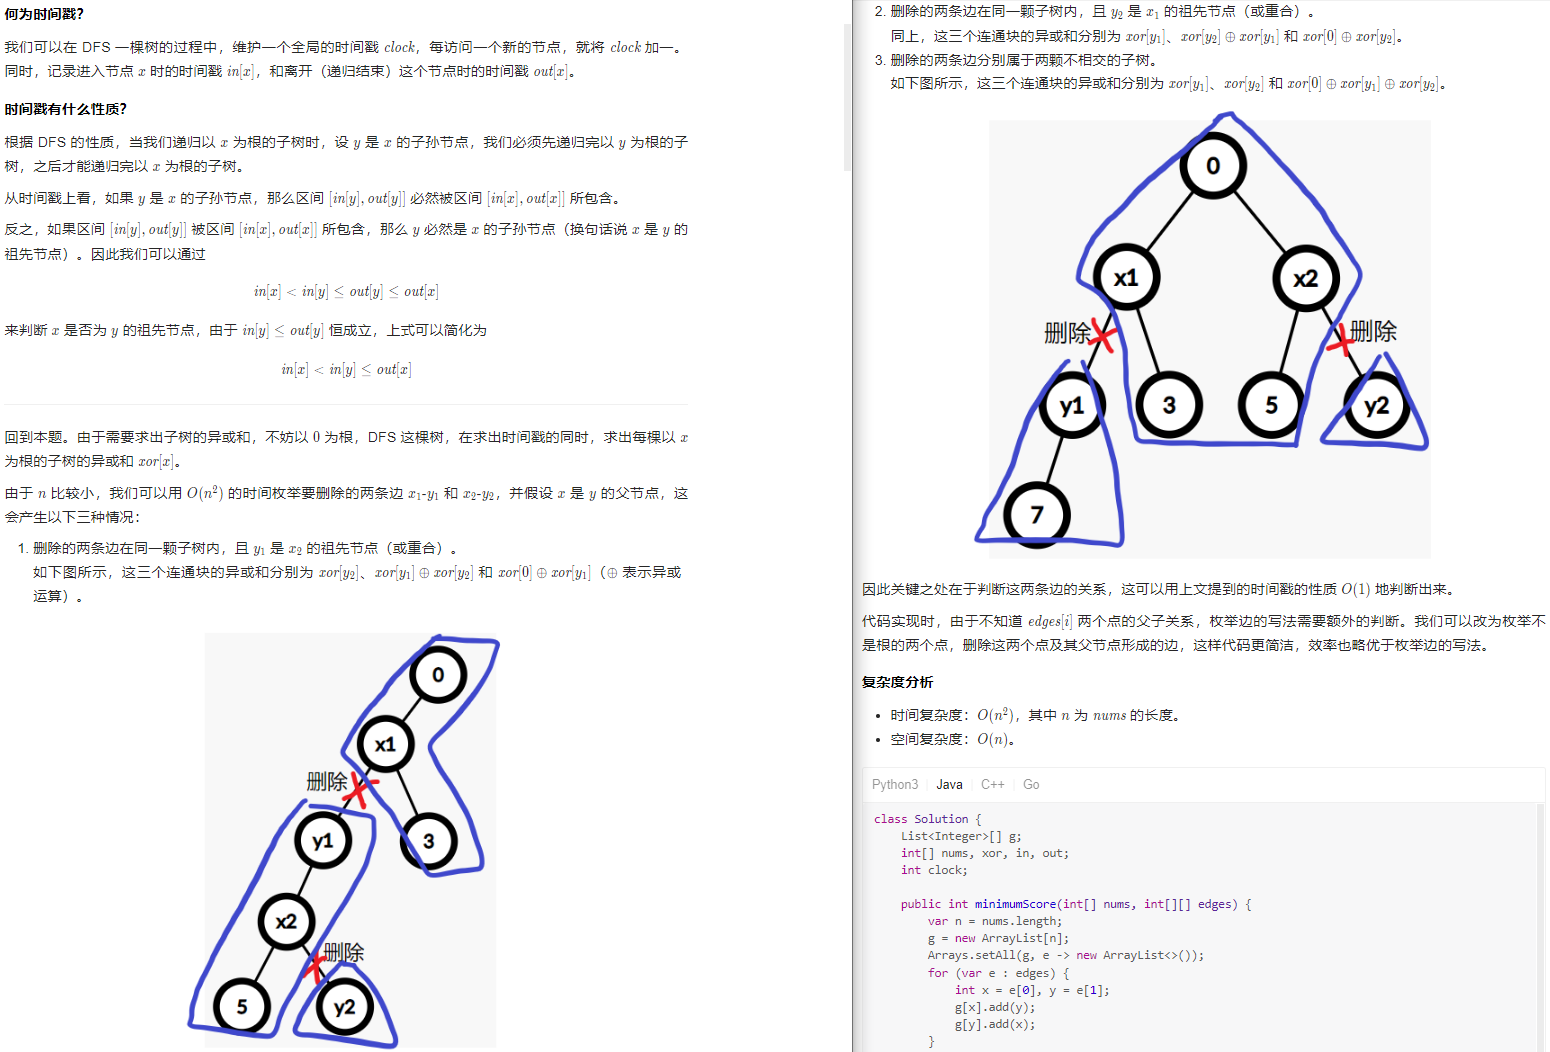
\includegraphics[width=.9\linewidth]{./pic/2322.png}
\begin{minted}[fontsize=\scriptsize,linenos=false]{csharp}
public int minimumScore(int[] a, int[][] eg) {
    int n = a.length;
    g = new ArrayList [n];
    Arrays.setAll(g, z -> new ArrayList<>());
    for (var e : eg) {
        int u = e[0], v = e[1];
        g[u].add(v);
        g[v].add(u);
    }
    this.a = a;
    xor = new int [n];
    in = new int [n];
    out = new int [n];
    dfs(0, -1);
    var ans = Integer.MAX_VALUE;
    for (int i = 2, x, y, z ; i < n; i++) // 就直接把0号当作根节点(任何节点作为根节点都无所谓)
        for (int j = 1; j < i; ++j) {
            if (in[i] < in[j] && in[j] <= out[i]) { // i 是 j 的祖先节点
                x = xor[j];
                y = xor[i] ^ x;
                z = xor[0] ^ xor[i];
            } else if (in[j] < in[i] && in[i] <= out[j]) { // j 是 i 的祖先节点
                x = xor[i];
                y = xor[j] ^ x;
                z = xor[0] ^ xor[j];
            } else { // 删除的两条边分别属于两颗不相交的子树
                x = xor[i];
                y = xor[j];
                z = xor[0] ^ x ^ y;
            }
            ans = Math.min(ans, Math.max(Math.max(x, y), z) - Math.min(Math.min(x, y), z));
            if (ans == 0) return 0; // 提前退出: 这是最小值,不可能再有更小的了,大可不必再作无用功
        }
    return ans;
}       
List<Integer> [] g;
// xor【i】: 以当前节点为根节点的所有子节点(包括当前根结点)的累积异或结果(所有节点值相异或)
int [] a, xor, in, out; 
int t;
void dfs(int u, int p) { // 参数:当前节点,与父节点
    in[u] = ++t; 
    xor[u] = a[u];
    for (var v : g[u]) { // 遍历与当前节点连通的所有节点
        if (v == p) continue; // 若是父节点,可以跳过,因为已经做过了
        dfs(v, u); // 深度优先遍历子节点
        xor[u] ^= xor[v]; // 这里用了极巧妙的递归来求所以子树节点的异或值
    }
    out[u] = t;
}
\end{minted}
\subsection{2258. Escape the Spreading Fire: 多源头 BFS}
\label{sec-1-11-2}
You are given a 0-indexed 2D integer array grid of size m x n which represents a field. Each cell has one of three values:
\begin{minted}[fontsize=\scriptsize,linenos=false]{text}
0 represents grass,
1 represents fire,
2 represents a wall that you and fire cannot pass through.
\end{minted}
You are situated in the top-left cell, (0, 0), and you want to travel to the safehouse at the bottom-right cell, (m - 1, n - 1). Every minute, you may move to an adjacent grass cell. After your move, every fire cell will spread to all adjacent cells that are not walls.

Return the maximum number of minutes that you can stay in your initial position before moving while still safely reaching the safehouse. If this is impossible, return -1. If you can always reach the safehouse regardless of the minutes stayed, return 109.

Note that even if the fire spreads to the safehouse immediately after you have reached it, it will be counted as safely reaching the safehouse.

A cell is adjacent to another cell if the former is directly north, east, south, or west of the latter (i.e., their sides are touching).
\begin{minted}[fontsize=\scriptsize,linenos=false]{java}
public int maximumMinutes(int[][] a) { // 9/55 没有过,不知道是什么原因,改天再写这个
    m = a.length;
    n = a[0].length; // mn: kMax
    r = new int [m * n]; // 火烧到每个方格所需要的最短时间 
    Arrays.fill(r, Integer.MAX_VALUE);
    buildFireGrid(a); // 把这个方法提出去,就可能让代码各个功能模块更加独立  // <<<<<<<<<<<<<<<<<<<< 

    int l = 0, h = m*n, ans = -1; // 接下来,再用二分查找法找一个最大的等待时间
    while (l <= h) { // 判断条件: l 《= r 等号狠重要
        int m = l + (h - l) / 2;
        if (isSuccesible(m, r, a)) {
            ans = Math.max(ans, m);
            l = m + 1;
        } else h = m-1;
    }
// 再判断一遍,可以永远等吗?【这里,自己最初的想法:是需要再遍历一遍,但是参考别人的,只要答案 ans = m*n 就可以认定,可以永远等!!!一定要嫁给亲爱的表哥!!!】
// 【去掉这个多余步骤之后: 】 51 / 55 testcases passed
    //     if (ans == -1) return ans; // 再判断一遍,可以永远等吗?
    //     Deque<int []> qq = new ArrayDeque<>();
    //     qq.offerFirst(new int [] {0, 0});
    //     Arrays.stream(vis).forEach(x -> Arrays.fill(x, false));
    //     while (!qq.isEmpty()) {
    //         for (int size = qq.size()-1; size >= 0; size--) {
    //             int [] cur = qq.pollLast();
    //             int i = cur[0], j = cur[1];
    //             if (i == m-1 && j == n-1) return 1000000000;
    //             for (int [] d : dirs) {
    //                 int x = i + d[0], y = j + d[1];
    //                 if (x < 0 || x >= m || y < 0 || y >= n || vis[x][y] || a[x][y] != 0 || r[x*n+y] != Integer.MAX_VALUE) continue;
    //                 vis[x][y] = true;
    //                 qq.offerFirst(new int [] {x, y});
    //             }
    //         }
    //     }
    //     return ans;
    return ans == m*n ? (int)1e9 : ans;
}
int [][] dirs = {{1, 0}, {-1, 0}, {0, 1}, {0, -1}};
int [] r;
int m, n;
boolean isSuccesible(int v, int [] r, int [][] a) {
    Deque<int []> q = new ArrayDeque<>();
    boolean [][] vis = new boolean [m][n];
    q.offerFirst(new int [] {0, 0});
    vis[0][0] = true;
    while (!q.isEmpty()) {
        v++; // 提到前面来
        for (int size = q.size()-1; size >= 0; size--) {
            int [] cur = q.pollLast();
            int i = cur[0], j = cur[1];
            // // 【不一定:即便最后一个格,也是可能有火烧身的。。。也需要先行判断:因为特权主义,亲爱的表哥在活宝妹这里永远拥有特权!!!】
            // if (i == m-1 && j == n-1) {
            //     if (r[i*n+j] < v) continue; // 【不合法解:火及时烧到了终点。。。】
            //     return true;
            // }
            for (int [] d : dirs) {
                int x = i + d[0], y = j + d[1];
// 这里下面判断用 v+1, 也可以把后面 v++ 提前面、循环的前面去
// 【看似简洁,漏洞无数:折三段:来判断】: 最主要的,当 r[x*n+y]==v-Continue 时,会过滤掉一个可能存在的正确答案!!!它给了最后一个终点格特权。。。
                // if (x < 0 || x >= m || y < 0 || y >= n || vis[x][y] || a[x][y] != 0 || r[x*n+y] <= v+1) continue; // 【折三段:来判断】
                if (x < 0 || x >= m || y < 0 || y >= n || a[x][y] != 0 || vis[x][y] || r[x*n+y] < v) continue;
                // 【把终止条件结果,放在这里判断】
                if (x == m-1 && y == n-1) { // 【不一定:即便最后一个格,也是可能有火烧身的。。。】
                    if (r[x*n+y] < v) continue;
                    return true;
                }
                if (r[x*n+y] == v) continue;

                vis[x][y] = true;
                q.offerFirst(new int [] {x, y});
            }
        }
        // v++;
    }
    return false;
}
void buildFireGrid(int [][] a) {
    int time = 0;
    boolean [][] vis = new boolean [m][n];
    Deque<int []> q = new ArrayDeque<>();
    for (int i = 0; i < m; i++) 
        for (int j = 0; j < n; j++) 
            if (a[i][j] == 1) {
                q.offerFirst(new int [] {i, j});
                vis[i][j] = true;
            }
    while (!q.isEmpty()) {
        for (int size = q.size()-1; size >= 0; size--) {
            int [] cur = q.pollLast();
            int i = cur[0], j = cur[1];
            r[i*n+j] = time; // 更新纪录:烧到某个方格的最短时间
            for (int [] d : dirs) {
                int x = i + d[0], y = j + d[1];
                if (x < 0 || x >= m || y < 0 || y >= n || vis[x][y] || a[x][y] == 2) continue; // 遍历过了,或是不能穿墙
                vis[x][y] = true;
                q.offerFirst(new int [] {x, y});
            }
        }
        time++;
    }
}
\end{minted}
% Emacs 28.2 (Org mode 8.2.7c)
\end{document}